
\documentclass[10pt, conference, compsocconf]{IEEEtran}

\usepackage{xcolor}
\usepackage{enumerate}
%\usepackage{enumitem}
\usepackage{amssymb}
\usepackage{graphicx}
\usepackage{subfigure}
\usepackage{url}
\usepackage{xspace}
\usepackage[hyperfootnotes=false,breaklinks]{hyperref}
\hypersetup{
	colorlinks,
	citecolor=red,
	linkcolor=blue,
	urlcolor=blue
}

%\newlength{\gapspace}
%\newcommand{\gap}[1][0cm]{\setlength{\gapspace}{#1}\vspace{.5\gapspace}\textbf{\color{red}[...]}\vspace{.5\gapspace}\xspace}

\newcommand{\NZ}[1]{\noindent\textcolor{blue}{\bf $\blacksquare$ Nannan: #1}}
\newcommand{\VT}[1]{\noindent\textcolor{orange}{\bf $\blacksquare$ Vasily: #1}}
\newcommand{\AB}[1]{\noindent\textcolor{red}{\bf $\blacksquare$ ARB: #1}}
\newcommand{\LR}[1]{\noindent\textcolor{cyan}{\bf $\blacksquare$ Lukas: #1}}
\newcommand{\DIM}[1]{\noindent\textcolor{olive}{\bf $\blacksquare$ Dimitris: #1}}
\newcommand{\alicomment}[1]{\noindent\textcolor{green}{\bf $\blacksquare$ Ali: #1}}

\newcommand{\abc}[1]{\noindent\textcolor{red}{\bf $\blacksquare$ AB: #1}}
\newcommand{\ie}{i.e.\ }
\newcommand{\eg}{e.g.,\ }
\newcommand{\etal}{et al.~}
\newcommand{\vs}{vs.\ }
\newcommand{\cf}{cf.~}

\newcommand{\sysname}{Slimmer}

% lukas: a more compact itemize/enumerate environment to save space and better looks
%\newenvironment{compactitemize}{%
%	\begin{itemize}[leftmargin=1em, itemsep=0em, parsep=0em, topsep=.1em, partopsep=.1em]}
%	{\end{itemize}}
%\newenvironment{compactenumerate}{%
%	\begin{enumerate}[leftmargin=1em, itemsep=0em, parsep=0em, topsep=.1em,partopsep=.1em]}
%	{\end{enumerate}}

\begin{document}
	
	%don't want date printed
	%\date{}
	
	%make title bold and 14 pt font (Latex default is non-bold, 16 pt)
	\title{
		%Registry Diet: Weight Loss Secrets for Docker Registry\\
		%Weight Loss Secrets for Docker Registry\\
		Slimmer: Weight Loss Secrets for Docker Registries
		%\\
		%Applying Deduplication to Docker Registry\\
		%Why and How to Apply Deduplication to Docker Registry
	}

%\usepackage{amsmath}
%\usepackage[normalem]{ulem}
%
%\usepackage{url}
%\usepackage{graphicx}
%\usepackage{epstopdf}
%\usepackage{xcolor}
%\usepackage{subfigure}
%
%\usepackage{xspace}
%\usepackage{latexsym}
%
%\usepackage[ruled,vlined]{algorithm2e}
%\usepackage{algorithmic}
%\usepackage{enumerate}

%\renewcommand\thefootnote{\textcolor{OrangeRed}{\arabic{footnote}}}
%\renewcommand\thefootnote{{\arabic{footnote}}}
%
%%\usepackage[anythingbreaks]{breakurl}
%\usepackage{wrapfig}
%\usepackage{layouts}
%\usepackage{setspace}
%\usepackage{blindtext}
%
%\usepackage{multirow}
%\usepackage{pifont}
%
%\usepackage{mathtools}
%\usepackage{relsize}
%\usepackage{ulem}
%\usepackage{comment}
%\usepackage{xifthen}
%\usepackage{footnote}


%\makesavenoteenv{tabular}
%\makesavenoteenv{table}
%
%\usepackage{caption}
%\DeclareCaptionType{copyrightbox}
%
%
%\DeclareCaptionFormat{myformat}{\hrulefill\\#1#2#3}
%\captionsetup[figure]{format=myformat}
%
%\usepackage{mathtools}
%
%\DeclarePairedDelimiter\abs{\lvert}{\rvert}%
%\DeclarePairedDelimiter\norm{\lVert}{\rVert}%

%\makeatletter
%\let\oldabs\abs
%\def\abs{\@ifstar{\oldabs}{\oldabs*}}
%%
%\let\oldnorm\norm
%\def\norm{\@ifstar{\oldnorm}{\oldnorm*}}
%\makeatother
%
%\newcommand*{\Value}{\frac{1}{2}x^2}%
%
%\usepackage{cleveref}
%
%\crefformat{section}{\S#2#1#3}
%
%\newcommand{\nancomment}[1]{\noindent\textcolor{red}{\bf Nannan: #1}}
%
%\newif{\ifSubmit}
%\newif{\ifFinal}
%\newif{\ifDraft}
%\Drafttrue
%%\Submittrue

%\ifSubmit
%\newcommand{\alicomment}[1]{}
%\newcommand{\yuecomment}[1]{}
%\else
%\newcommand{\alicomment}[1]{\noindent\textcolor{blue}{\bf Ali: #1}}
%\newcommand{\arbcomment}[1]{\noindent\textcolor{red}{\bf arb: #1}}
%\newcommand{\yuecomment}[1]{\noindent\textcolor{red}{\bf Yue: #1}}
%\fi
%%
%%
%%\newcommand{\Comment}[1]{{{\color{red}#1}}}
%%\newcommand{\tobeadded}[1]{{{\color{blue}#1}}}
%\newcommand{\myparagraph}[2][]{\ifthenelse{\isempty{#1}}{\vspace{0.02in}\noindent\textbf{#2}}{\vspace{-0.02in}\noindent\textbf{#2}}}
%%
%\newcommand{\proj}{Chameleon}
%%
%\usepackage{booktabs}
%\newcommand{\otoprule}{\midrule[\heavyrulewidth]}
%
%\newcommand{\ie}{i.e.\ }
%\newcommand{\eg}{e.g.\ }
%\newcommand{\etal}{et al.~}

%
%\begin{document}
%
%\title{{\proj}: An Adaptive Wear Balancer for Flash Clusters}

%\author{
%	{\rm Nannan Zhao$^{1}$,
%		Vasily Tarasov$^{2}$,
%		Ali Anwar$^{1}$},
%	{\rm Lukas Rupprecht$^{2}$, 
%		Dimitrios Skourtis$^{2}$,}\\
%	{\rm Amit S. Warke$^{2}$,
%		Mohamed Mohamed$^{2}$, 
%		Dean Hildebrand$^{2}$\thanks{Now at Google.}, and Ali R. Butt$^{1}$}\\
%	{{$^1$}{Virginia Tech}, {$^{2}$}{IBM Research---Almaden}}
%}

\maketitle


\begin{abstract}

Docker containers have become the de facto standard for supporting modern enterprise applications due to the highly desirable features of 
isolation, low overhead, and efficient packaging of the execution environment.
%
Containers are created from images that preserve software dependencies,
environment configuration, and other parameters that affect the application's
runtime.
%
Docker allows sharing of such images between users via a Docker registry. 
%
The amount of data Docker registries store is massive; for instance, Docker Hub---a popular public registry---
stores at least a half million public images.
%
%As the amount of images stored in public and private Docker registries
%increases it becomes important to study images' characteristics.
%
%
Investigating the storage-centric properties of containerized applications can reveal useful insights and findings that can enable new optimizations, higher performance, and identification of bottlenecks. 
The massive Docker Hub  dataset of over 50~TB thus offers a unique opportunity for such an endeavor, which we undertake in this paper. We perform the first in-depth analysis of a large scale Docker registry.  
%
%Our goal is to collect statistics from a large amount of Docker images and
%perform a large-scale characterization of Docker images.
%
We characterize images using multiple metrics, e.g., image size distribution,
file size and type distribution, the number of layers per image, the amount of
redundant data between images and layers.
%
\abc{add an example or two of the key findings?\nancomment{added findings to the end of intro}}
%
Our findings help to make conscious decisions when designing storage for
containers and Docker in particular.
 
\end{abstract}

\section{Introduction}

Because of their lightweight isolation and fast deployment,
\emph{containers}~\cite{process-containers-linux} have recently gained a
significant traction.
%
Polls suggest that 87\% of enterprises are at various stages of adopting
containers, and they are expected to constitute a lucrative \$2.5 billion
market~\cite{container-grow-by2020} by 2020.

Docker combines process containerization with efficient and effective packaging
of complete runtime environment in so called {\em images}.
%
Images are composed of shareable and {\em content addressable layers}.
%
Each layer is essentially a set of files that 
are compressed in a single archive.
%
Both images and layers are stored in Docker registry and accessed by clients as
needed.
%
Since layers are uniquely identified by using collision-resistant hash of the
content, no duplicate layers are stored in Docker registry.

Currently, registry is growing rapidly.
%
For example,   Docker Hub~\cite{docker-hub}, the most widely used registry,
stores more than 500,000 public image repositories comprising of over 2 million
layers.
%
The size of the registry continues to steadily increase---we observed a
linear growth of the number of images in Docker Hub over a period from June to
September 2017, with an average creation rate of 1,241 repositories per day.
%
%(as shown in Figure~\ref{fig_image_growth}.
%
This massive image dataset that presents challenges to the registry storage
infrastructure has remained a largely unexplored area.

In this paper, we performed the first, in-depth, large-scale redundancy
analysis of the images and layers stored in the Docker Hub
registry~(\S\ref{sec:background}).
%
We downloaded 51TB worth of Docker Hub images which contains over 5 billion (167 TB)
of files after decompression.
%
%We started our analysis
%with collecting all the metadata over xxx images and  conducted the first
%comprehensive characterization of the image dataset (or union file systems). This analysis is particularly useful as no prior work exists on union file
%systems~\cite{xxx} and dataset used and created exclusively for Docker,
%which are different from either analysis on EX4 linux file system~\cite{xxx} or
%Windows file system~\cite{xxx}.
%%
%%We not only present the distribution for each metric but also pointed out the
%%challenges faced by Docker engine designer and registry designer based on
%%global knowledge (or analysis) of metadata. 
%We also provide useful insights (parameters or metrics)
%for the developers to better
%understand the file systems used by Docker container. 
%
%%Unfortunately, it's unknown whether  this coarse-grain layer-level content
%%addressable storage (LLCAS) can efficiently reduce duplicates, and how much
%%redundant data is stored in layer, image, and registry because there is no
%%prior research on registry dataset analysis.
%
%We continued with the deduplication analysis of the dataset.
%
Surprisingly, we found only around 3\% of the containing files are unique files
while others are redundant copies, which means that current layer-level content
addressable storage cannot efficiently reduce duplicates.
%
To inspect what are the redundant files and why there are so many redundant
files, we conducted a comprehensive redundancy analysis on the 167 TB
uncompressed dataset.
%
We made three major observations.
%
\begin{compactitemize}
%
\item Only 10\% of layers are referred by more than one images, 
meaning that layer-level content addressability is not efficiently utilized by Docker registry.
%
\item A large amount of full file duplicates are shared cross layers and cross images. 
Only 3\% of files in the uncompressed layer dataset are unique files while others are redundant file copies.
%
\item Majority of the file duplicates are executables and object files, which are mostly created by the source code duplicates.
%
We found that different Docker developers are prone to replicate same source codes from external public repositories (e.g., GitHub~\cite{xxx}) and store these source code duplicates cross layers because there is no official images available for pulling.  

\end{compactitemize}

Finally, we proposed a file-level content addressable storage model (FLCAS) for Docker registry, which utilizes file-level deduplication to remove redundant files. 
%
We simulated FLCAS for 0.9 million layers and provided different suggestions to improve deduplication performance. The simulation result shows that (1) processing layers in parallel can largely improve throughput. For example, 80\% of file-level deduplication time is
less than 9.09 s per layer and by processing 60 layers in parallel, our one-node file-level deduplica-
tion prototype can process about 3 layers per second.
(2) Fast compression methods can mitigate pulling overhead caused by re-compression  because files are required to be re-compressed as a compressed layer archival file to serve the incoming pulling requests.


%%%%%%%%%%%%%%%%%%%%%%%%%%%%%%%%%%%%%%%%%%%%%%%%%%%%%%%%%%%%%%%%%%%%%%%%%%%%%%
%                                                                            %
%                                OLD INTRO                                   %
%                                                                            %
%%%%%%%%%%%%%%%%%%%%%%%%%%%%%%%%%%%%%%%%%%%%%%%%%%%%%%%%%%%%%%%%%%%%%%%%%%%%%%

%Finally, we proposed and implemented Docker registry design that performs
%deduplication.
%%
%In our thorough redundant analysis and characterization of the xxxx images,
%with xxxx layers and xxxx files, we investigated the following four research
%questions (RQs):
%
%\begin{compactitemize}
%%
%\item How much redundant data stored in layers, images, and registry? Although
%layer-level address content addressable storage is adopted by Docker, we do not
%know whether  this coarse-grain layer-level content addressable storage (LLCAS)
%can efficiently reduce duplicates, and how much redundant data is stored in
%layer, image, and registry.
%%
%\item What are the redundant files and why there are so many redundant files?
%We aim to identify what are the redundant files that users mostly replicate.
%%
%Such information will provide Docker designer knowledge (user behavior) to
%better develop and optimize Docker container and Docker registry storage
%system.
%%
%\item What are the challenges faced by Docker registry and engine designer? By
%characterizing and analysis all the image metadata, we aim to identify the
%challenges' faced by registry designer and guide designers'optimization and
%users' development.
%%
%\item How to reduce the redundant files? We aim to propose a file-level content
%addressable model to reduce the redundant files by using file-level dedup while
%maintaining a good performance.
%%
%\end{compactitemize}
%
%The significance of this work are (1) our empirical evidence that large amount
%of redundant files exist in layers, images, and registry and layer-level
%content addressable storage is not efficient to remove redundant files;(2)
%findings about what are the redundant files and why there are so many redundant
%files exist;(3) first in-depth characterization on image dataset (union file
%systems)(4) a file-level content addressable model that can efficiently remove
%redundant copies while maintain a good performance.

%For years, virtual machines served as a cornerstone of computing resource
%virtualization both on premises and in the cloud~\cite{rosenblum2005virtual}.
%%
%Recently, however, \emph{container-based} virtualization started to gain
%significant traction~\cite{process-containers-linux}.
%%
%According to polls, over 87\% of enterprises are at various stages of adopting
%containers; analysts also predict that by 2020, containers will constitute a
%lucrative \$2.5 billion market~\cite{container-grow-by2020}.
%
%
%
%At its core, container is a set of processes which are isolated by the operating
%system kernel in terms of visibility and resources. This allows containers to share
%the same kernel without being aware of each other.
%%
%For example, Linux performs visibility isolation (for user identifiers, file systems,
%network, etc.) using namespaces~\cite{man-namespaces} and enforces resource
%utilization constraints with control groups~\cite{kernel-doc-cgroups}.
%%
%Compared to virtual machines, containers use less memory and storage, are much
%faster to start, and typically cause less execution
%overhead~\cite{felter2015updated, Disco, HypervisorsvsLightweight}.
%
%The rapid increase in use of container technology was largely made possible by
%container management frameworks, with Docker being one of the most popular
%solutions~\cite{docker}.
%%
%Docker combines process containerization with efficient and effective runtime
%environment packaging.
%%
%Software is packaged in container \emph{images}, each consisting of several
%read-only \emph{layers} and a manifest which describes container metadata, \eg
%what layers make up an image and which command to run at container startup.
%%
%Read-only layers can be shared between different images and encapsulate
%file-system trees for dockerized processes.
%
%%Docker is another technology whose popularity grew rapidly in the recent
%%years~\cite{docker}.
%%
%%When Docker starts a container, it combines read-only layers (and an additional
%%writable layer to store changes) into a single namespace and starts the process
%%declared in the manifest in the new namespace~\cite{docker-driver-eval}.
%
%
%
%Docker images are stored in a centralized \emph{registry} and are pushed to and
%pulled from the registry by clients as needed.
%%
%Docker Hub~\cite{docker-hub} is the most widely used Docker registry
%installation which, according to our estimates, stores more than 400,000
%\emph{public} image repositories comprising a total of 2 million layers.
%%
%This amount is steadily increasing and we observed a linear growth of the
%number of images over a period from June to September 2017.
%
%
%
%While this massive dataset presents challenges to the registry storage
%infrastructure, it also provides opportunities to better understand how
%containers are used in practice.
%%
%Currently, there is little known about the contents, use cases, and workloads
%of production containers.
%%
%In part, this is due to the privacy concerns that organizations and individuals
%have when sharing details of their computing environments.
%%
%However, this knowledge is imperative to design and evaluate novel approaches
%to improve the performance and reliability of containers.
%
%
%
%
%In particular, storage for containers has remained a largely unexplored
%area~\cite{login-container-storage-options}.
%%
%We believe one of the prime reasons is the limited understanding of what data
%is stored inside containers.
%%
%This knowledge can not only help to directly improve the registry and container
%storage infrastructure but also allows to infer container use cases and derive
%representative workloads from that.
%%
%While existing work as focused on various aspects of
%containerization~\cite{slacker, dockervulnerabile, dockerfinder, analysisdockergithub, dockerssd}, analyzing the
%contents of images and layers has not received much attention.
%
%
%
%
%%Though much research was focused on various aspects of
%%containerization~\cite{prev-work-1, prev-work-2, prev-work-3}, storage for containers
%%remains an unexplored territory~\cite{login-container-storage-options}.
%%
%%To start designing a novel storage solution for containers,
%%or to optimize and fairly evaluate existing ones,
%%it is imperative to understand containers' real-world
%%use cases and workloads in sufficient details.
%%
%%Unfortunately, little is known about how containers are used in the real world.
%%
%%In part, this is due to the privacy concerns that organizations and individuals
%%have when sharing details of their computing environments.
%
%
%%Docker images are stored at the centralized \emph{registry} and are pushed to
%%and pulled from the registry by clients as needed. 
%%
%%The most known Docker registry installation is Docker Hub which according to
%%our estimates stores at least 400,000 \emph{public} images that consist of at
%%least 2,000,000 layers.
%
%
%
%
%In this paper we perform the first, comprehensive, large-scale characterization of
%Docker registry contents.
%%
%We downloaded over 50TB of Docker images from Docker Hub and analyzed
%traditional storage properties---\eg, file sizes and types, data compression
%ratios, directory depths---as well as Docker-specific properties---e.g., the number
%of layers per image and the amount of layer sharing.
%%
%%Our insight in this study is that this massive dataset can be used to understand what
%%applications run in containers, how much data they store, and the properties of
%%the data.
%%
%We found, for example:
%\begin{compactenumerate}
%	\item 90\% of the repositories only have a very small pull count (less than 333), which suggests that Docker hub is a good fit for caching few popular repositories or images.
%	\item majority of the images and layers in Docker hub have a smaller size. 90\% of images can be compressed with less than 500 MB and 70\% of images are less than 500 MB even without compression. 90\% of layer can be compressed with less than 63 MB and 77\% of layers are less than 63 MB even without compression.
%	\item Docker images has a great potential for compression to save space.
%	\item 90\% of images have less than 18 layers. Half of images have less than 8 layers. 
%	\item 10\% of layers are referenced more than one image.
%	\item Around 90\% of layers' directory depth is less than 30. 50\% of layers' directory depth is less than ~3.
%	\item Around 30\% of files are ASCII text files. 
%	About 11\% files are gzip compressed files 
%	Interestingly, about 1\% of files are empty. 
%\end{compactenumerate}
%%
%\vcomment{Here we need to stick an example or two of interesting findings. \nancomment{addressed}}
%
%%From our findings, we infer a set of propositions to describe how Docker is
%%used in the real world:
%%\lrcomment{Can we summarize our findings in a few propositions to put here?}.
%%
%%We believe our findings will improve the understanding of containers' data and lay
%%a solid ground for future storage optimizations at clients and registries in
%%Docker and beyond.
%
%After introducing the Docker background~(\S\ref{sec:background}),
%this paper makes the following contributions:
%\begin{compactenumerate}
%  \item We describe a comprehensive methodology to retrieve the complete set of
%  	images stored in Docker Hub~(\S\ref{sec:methodology});
%  \item We perform the first in-depth analysis of container images stored in
%    Docker Hub~(\S\ref{sec:char}).
%%  \item based on our analysis, we formulate propositions on how Docker is currently
%%    used to help guide optimizations and benchmark
%%    workloads~(\S\ref{sec:propositions}).
%\end{compactenumerate}
%
%After discussing related work~(\S\ref{sec:related}),
%the paper concludes~(\S\ref{sec:conclusion}).
%
%%The rest of the paper is organized as follows. We explain
%%relevant Docker details in Section~\ref{sec:background} and our methodology in
%%Section~\ref{sec:methodology}. We present dataset characterization in
%%Section~\ref{sec:results}, describe related work in Section~\ref{sec:related},
%%and conclude in Section~\ref{sec:conclusion}.

\section{Docker Registries}
\label{sec:background}

%\paragraph{Docker registry.}

%A Docker image consists of an ordered series of \emph{layers}.
%
%Each Docker layer contains a subset of the files in the image and often
%represents a specific component/dependency of the image, \eg a shared library.
%
%Layers can be shared between two or more images if the images depend on the
%same layer.

In this section, we explain how the existing Docker registry works and how users
can interact with it.
%
The main purpose of a registry is to store container images and make them available
to other users.
%
Therefore, it allows Docker clients to \emph{push} images to and \emph{pull}
images from the registry.
%
A number of public Docker registry deployments
exist~\cite{docker-hub,amazon-ecr,jfrog-artifactory,azure-cr,google-cr} and
enterprises often resort to running private registries for improved security
and privacy.
%
The Docker community specifies the REST API for clients to communicate with the
registries~\cite{docker-registry-api} and provides a reference registry server implementation~\cite{docker-registry-software} which serves as
a basis for commercial deployments.





Docker registries group images in \emph{repositories}, each containing
different versions (\emph{tags}) of the same image, identified as
\texttt{<repo-name:tag>}.
%
For each tagged image in a repository, the Docker registry stores a \emph{manifest}.
%
The manifest is a JSON file, which contains the runtime configuration for a
container image (\eg environment variables) and the list of layers which make
up the image.
%
A layer is stored as a compressed archival file and identified using a digest that is computed as a hash (SHA-256) over
the uncompressed content of the layer.
%
When pulling an image, a Docker client first downloads the manifest and then the
layers referenced in it (unless the layers are already present on the client).
%
When pushing an image, a Docker client first uploads the layers (if not already present in
the registry) and then uploads the manifest.





The current Docker registry software is a single-node application.
%
To scale the registry and serve many requests concurrently, organizations typically deploy a load
balancer like NGINX in front of several independent registry
instances~\cite{dockerworkload, anwar-cloud19}.
%
All the instances delegate storage and retrieval of images to drivers that interact with
either a locally mounted shared file system or a remote object storage~\cite{s3,azure,swift,aliyun}.
%
%For example, the Google Container Registry~\cite{GoogleContainerRegistry} uses
%Google cloud as its backend image store.
%
Upon a \texttt{PUT} layer request from a Docker client, the Docker registry receives the layer and forwards it to the
backend storage driver.
%
Typically, multiple replicas of the layer are stored for redundancy.
%
Subsequent \texttt{GET} layer requests can be served by any registry server,
which will get the layer from the backend storage using the configured driver.

% that hold a replica of that layer.
%
%Service providers often use geographically distributed registries for faster
%access, e.g., IBM's Container Registry setup spans five
%regions~\cite{dockerworkload}. 


%\paragraph{Deduplication} Most existing cloud storage providers employ data
%deduplication techniques to eliminate redundant data, same data stored more
%than once.
%
%Deduplication techniques significantly reduce storage needs and therefore
%reduce storage costs and improve storage efficiency.
%
%Data deduplication works by storing duplicate data chunks only once, keeping
%only the unique data chunks. 
%
%Current cloud providers deploy a cross-user client-side fixed-size-chunk-level
%data deduplication that delivers the highest deduplication
%gain~\cite{pooranian2018rare}.
%
%These approaches maximize the benefit of deduplication: The cross-user data
%deduplication treats cloud storage as a pool shared by all the cloud users,
%because the potential for data deduplication is the highest as the probability
%for redundancies and duplicates is higher the more inclusive the shared pool.
%
%The fixed-size-chunk-level specifies that a fixed-size chunk is the unit for
%checking for duplicates on cloud storage.
%
%Google cloud and AWS employ StorReduce, a deduplication software that performs
%in-line data deduplication transparently and resides between the client's
%application and the hosting cloud storage.
%
%StorReduce provide 80-97\% storage and bandwidth reduction to the cloud
%providers~\cite{StorReduce_google}.

%
\section{Methodology}
\nancomment{
	outline: \\
	1. our method to collect and download images \\
	(how, pull, extracting, manifest+layer tarball, server setup) \\
	2. our Dataset \\
	(size, table)
}

Our methodology has two steps. First, We massively download the Docker images from Docker registry. Then we analyze the Docker images we download. Instead of using Docker (or Docker engine) to download Docker images, we wrote our own downloader that utilizes Docker Registry API to simultaneously download \textbf{original} manifests, config files, and layer tarballs. One reason is that docker engine will automatically convert the manifests from lower version (Schema 1) to higher Schema (Schema 2), which affects our result about manifest version statistics; the other reason is that layer content directories are not visible for some docker storage drivers, e.g., devicemapper, which is difficult to profile the layer content. Overall, We downloaded XXX Docker image with XXX Docker layers. Table~\ref{XXX} summaries the statistics of Docker image dataset we downloaded. Then, we profiled the layers, config files, and manifests we downloaded and calculated the statistic distribution for different metrics. 


\subsection{Downloader}

Our downloader is a python script that can download multiple images simultaneously and during each image downloading process, layers are downloaded in parallel. To download the original manifests, config files, and layer tarballs from Docker registry, downloader embeds a Docker registry client API~\cite{xxx} which only encapsulates manifest, config file and layer downloading functions in Docker engine without extracting layer tarball and converting manifest version. 

To download a Docker image, the image's name and tag should be provided. To the best of our knowledge, Docker Hub doesn't provide a method to list their public images. Public Docker images stored in Docker registry can be divided into official images and non-official images. The number of Official images is only xxx. While estimating and obtaining all the non-official images requires crawling Docker Hub. We created Crawler to crawl Docker Hub websites, parse the website source code and get a list of public both official and non-official images.

\subsubsection{Crawler}

Docker Hub website provides search service for users to search for a specific docker image or a list of Docker images that contains a specific word/string. Each public non-official Docker image shown on the website is comprised of namespace (i.e., user name), `/', and repository name. In this case, we search for '/' and get a list of images which contains '/'. In other words, this method lists all the non-official images stored in Docker Hub. Then, crawler crawls the websites that contains search results, parses the website source code and get the list of non-official images'names. 

A interesting observation is that we can get a similar list of images if we replace '/' with '*'. Note that from 5/30/2017-7/11/2017, we used this method to obtain the total amount of images stored in Docker Hub. But after 7/11/2017, the website shows nothing when we search for '/' for some unknown reasons. Hence, now we can search for '*' instead of '/' to get a list of Docker images.

%The name space for official images is library. For example, official image redis's name is library/

\subsubsection{Downloading the images}

As shown in Figure~\ref{}, the downloader first obtains a list of images through crawling Docker Hub. Then, it build

\subsubsection{Docker image dataset statistics}

We ran Crawler first and got a list of Docker images on 5/30/2017. The amount of both official and non-official images we got is xxx. However, there are duplicated image names in the list. The reason probably is that Docker Hub adjusted websites'order or modified the websites because of the increasing of Docker images during our crawling process. Our crawler has a unavoidable delay between each HTTP requst and HTTP response. So it couldn't reflect the websites'order or website content changes. After reducing the repeated images, we got xxx distinct images totally. 

Then we started downloading process to download those images. It took roughly 30 days to finish. Overall, we downloaded xxx images with xxx layers as shown in Table~\ref{XXX}. There are xxx of images we couldn't download. There are two reasons: first, around xxx of images were either deleted or empty. Second, around xxx of images doesn't have tag:latest. As we discussed before, we only downloaded the images with latest version.

%Some embedded literal typset code might 
%look like the following :
%
%{\tt \small
%\begin{verbatim}
%int wrap_fact(ClientData clientData,
%              Tcl_Interp *interp,
%              int argc, char *argv[]) {
%    int result;
%    int arg0;
%    if (argc != 2) {
%        interp->result = "wrong # args";
%        return TCL_ERROR;
%    }
%    arg0 = atoi(argv[1]);
%    result = fact(arg0);
%    sprintf(interp->result,"%d",result);
%    return TCL_OK;
%}
%\end{verbatim}
%}
%
%Now we're going to cite somebody.  Watch for the cite tag.
%Here it comes~\cite{Chaum1981,Diffie1976}.  The tilde character (\~{})
%in the source means a non-breaking space.  This way, your reference will
%always be attached to the word that preceded it, instead of going to the
%next line.
%\section{Characterization}
\label{sec:char}

In this section we perform storage-oriented characterization of the Docker Hub
dataset and draw our insights.
%
After presenting registry growth trends, we characterize layers
(\S~\ref{sec:layers}) and then proceed to images (\S~\ref{sec:images}).
%
\paragraph{Docker Hub growth.} Figure~\ref{fig_image_growth} shows the total
number of repositories in Docker Hub from May 30 to September 20, 2017.
%
%As discussed in~\cite{XXX}, Crawler searched for `/' by using Docker hub
%search engine, crawled the web page, and obtained the total number of
%non-official public repositories in Docker hub each day. By summing both
%official repository count and non-official repository count, we got the total
%number of repositories in Docker hub each day.
%
During this 110-day period the total number of repositories increased from
633,915 to 687,292, resulting to 1,241 repositories created per day on average.
%
The graph is missing the points for the July 11 to July 26 because Docker Hub
stopped indexing ``/'' symbol in the repository names (which we originally used
to search for repositories).
%
We noticed this issues on July 26 and started to use ``*'' symbol for search
instead.


\begin{figure}
  \centering
  \includegraphics[width=0.5\textwidth]{graphs/image_growth.pdf}
  \caption{Total number of public repositories in Docker Hub
	   from May 30 to September 20, 2017. Y axis starts
	   at 630,000 repositories.
	   \vcomment{X axis label should be ``Date''.}
	   \vcomment{Y axis label x100,000 ``is badly aligned''.}
	   \vcomment{Y axis label x100,000 ``is badly aligned''.}
	  }
  \label{fig_image_growth}
\end{figure}

\subsection{Layers}
\label{sec:layers}

\paragraph{Layer size}

\begin{figure}[!t]
	\subfigure[CDF of layer size]{\label{fig_layer_size}
		\includegraphics[width=0.4\textwidth]{graphs/layer-size-cdf.pdf}
		}
		\centering
		\subfigure[CDF of image size]{\label{fig_image_size}
			\includegraphics[width=0.4\textwidth]{graphs/image-size-cdf.pdf}%
			}
			
			\caption{Image/layer size distribution}
			\label{fig:image-layer-size}
			\end{figure}

\paragraph{Layer directory depth}
%\nancomment{fs metadata overhead}

\begin{figure}[!t]
	\centering
	\subfigure[CDF of layer depth]{\label{fig_reference_cnt_cdf}
		\includegraphics[width=0.21\textwidth]{graphs/layer-depth-cdf.pdf}%
	}
	\subfigure[Histogram of layer depth]{\label{fig_reference_cnt_pdf}
		\includegraphics[width=0.21\textwidth]{graphs/layer-depth-pdf.pdf}
	}
	\caption{Layer depth distribution}
	\label{fig:reference-cnt}
\end{figure}

\paragraph{Directory count and File count}
%\nancomment{how union fs handle so large dirs}
\begin{figure}
	\centering
	\includegraphics[width=0.4\textwidth]{graphs/dir-cnt-cdf.pdf}
	\caption{CDF of directory count per image/layer.
	}
	\label{fig:reference-cnt}
\end{figure}

\begin{figure}[!t]
	\centering
	\subfigure[Histogram of directory count per image]{\label{fig_reference_cnt_cdf}
		\includegraphics[width=0.2\textwidth]{graphs/image-dir-cnt-pdf.pdf}%
	}
	\subfigure[Histogram of directory count per layer]{\label{fig_reference_cnt_pdf}
		\includegraphics[width=0.22\textwidth]{graphs/layer-dir-cnt.pdf}
	}
	\caption{Histogram of directory count distribution}
	\label{fig:reference-cnt}
\end{figure}

Next, we look at the directory (Figure~\ref{fig-dir}) and file count
(Figure~\ref{fig-file}) in images to determine if deploying images requires
handling of large amounts of metadata. Looking at directories, we see that 90\%
of images have less than 7,344 directories while the median is at 296. For
files, 90\% of images have less than 64,780 files with a median of 1,090.

This is consistent with our analysis of layer-based file and directory counts
and the number of layers per image. Again, we conclude that most images do not
require an extensive amount of metadata when being deployed as file and
directory counts are low except for few outliers.

\paragraph{File count} 
%\nancomment{still metadata overhead}
\begin{figure}
	\centering
	\includegraphics[width=0.4\textwidth]{graphs/file-cnt-cdf.pdf}
	\caption{CDF of file count per image/layer.
	}
	\label{fig:reference-cnt}
\end{figure}

\begin{figure}[!t]
	\centering
	\subfigure[Histogram of directory count per image]{\label{fig_reference_cnt_cdf}
		\includegraphics[width=0.21\textwidth]{graphs/image-file-cnt-pdf.pdf}%
	}
	\subfigure[Histogram of directory count per layer]{\label{fig_reference_cnt_pdf}
		\includegraphics[width=0.22\textwidth]{graphs/layer-file-cnt-pdf.pdf}
	}
	\caption{Histogram of directory count distribution}
	\label{fig:reference-cnt}
\end{figure}

Lastly, we look at file and directory metrics in layers.
Figure~\ref{fig_file_cnt} and~\ref{fig_dir_cnt} show the CDFs of file and
directory counts in all layers, respectively.
%
The results show that 90\% of layers contain less than 7,410 files while half
of the layers have less than 30 files.
%
We also found that 27\% of the layers only have a single file while 7\% even
showed no files at all. We currently do not know the exact reason for the
layers without files, but one theory is that these layers use Docker volumes to
store all requred files (including executables).
% plan to investigate their corresponding images in the future.
%\nancomment{The layers are not empty since it could have directories}.
On the other hand, the largest layer contains 826,196 files and was part of a
Debian image.
%
%The average is 2,200.
%
For directories, 90\% of the layers have less than 826 directories and half of
the layers consist of less than 11 directories. We again observe a wide range
with a minimum of a single directory and a maximum of 111,940. The layer with
the most directories was part of the \textit{conjurinc/developer-quiz} image.

%\paragraph{Directory depths}

%After extracting and unpacking gzip compressed layer archival files,
Besides the count, we also calculate the maximum directory depth for each layer
(Figure~\ref{fig_layer_depth}).
%
Around 90\% of all layers have a directory depth less than 10 while for 50\% of
the layers, the directory depth is less than 4. 
%
The most frequent directory depth is 3 with 313,000 layers showing this depth
value (Figure~\ref{fig_hist_layer_depth}).
%
%About 313,000 layers' layer directory depth is 3, which is the peak value in
%the figure.
%
%The maximum repeat count is 444 while the median is 4. The average is ~5.

This analysis shows that the majority of layers consists only of a small number
of files and does not contain deeply nested directory hierarchies. Hence,
except a few outliers, unpacked layers do not require a large amount of
metadata from the storage system.
\subsection{Images}
\label{sec:images}

Next, we study images in terms of their popularity, size and their use of layers.

\begin{figure}[!t]
	\centering
	\subfigure[CDF of repositories by pull count]{\label{fig_pull_cnt_total}
		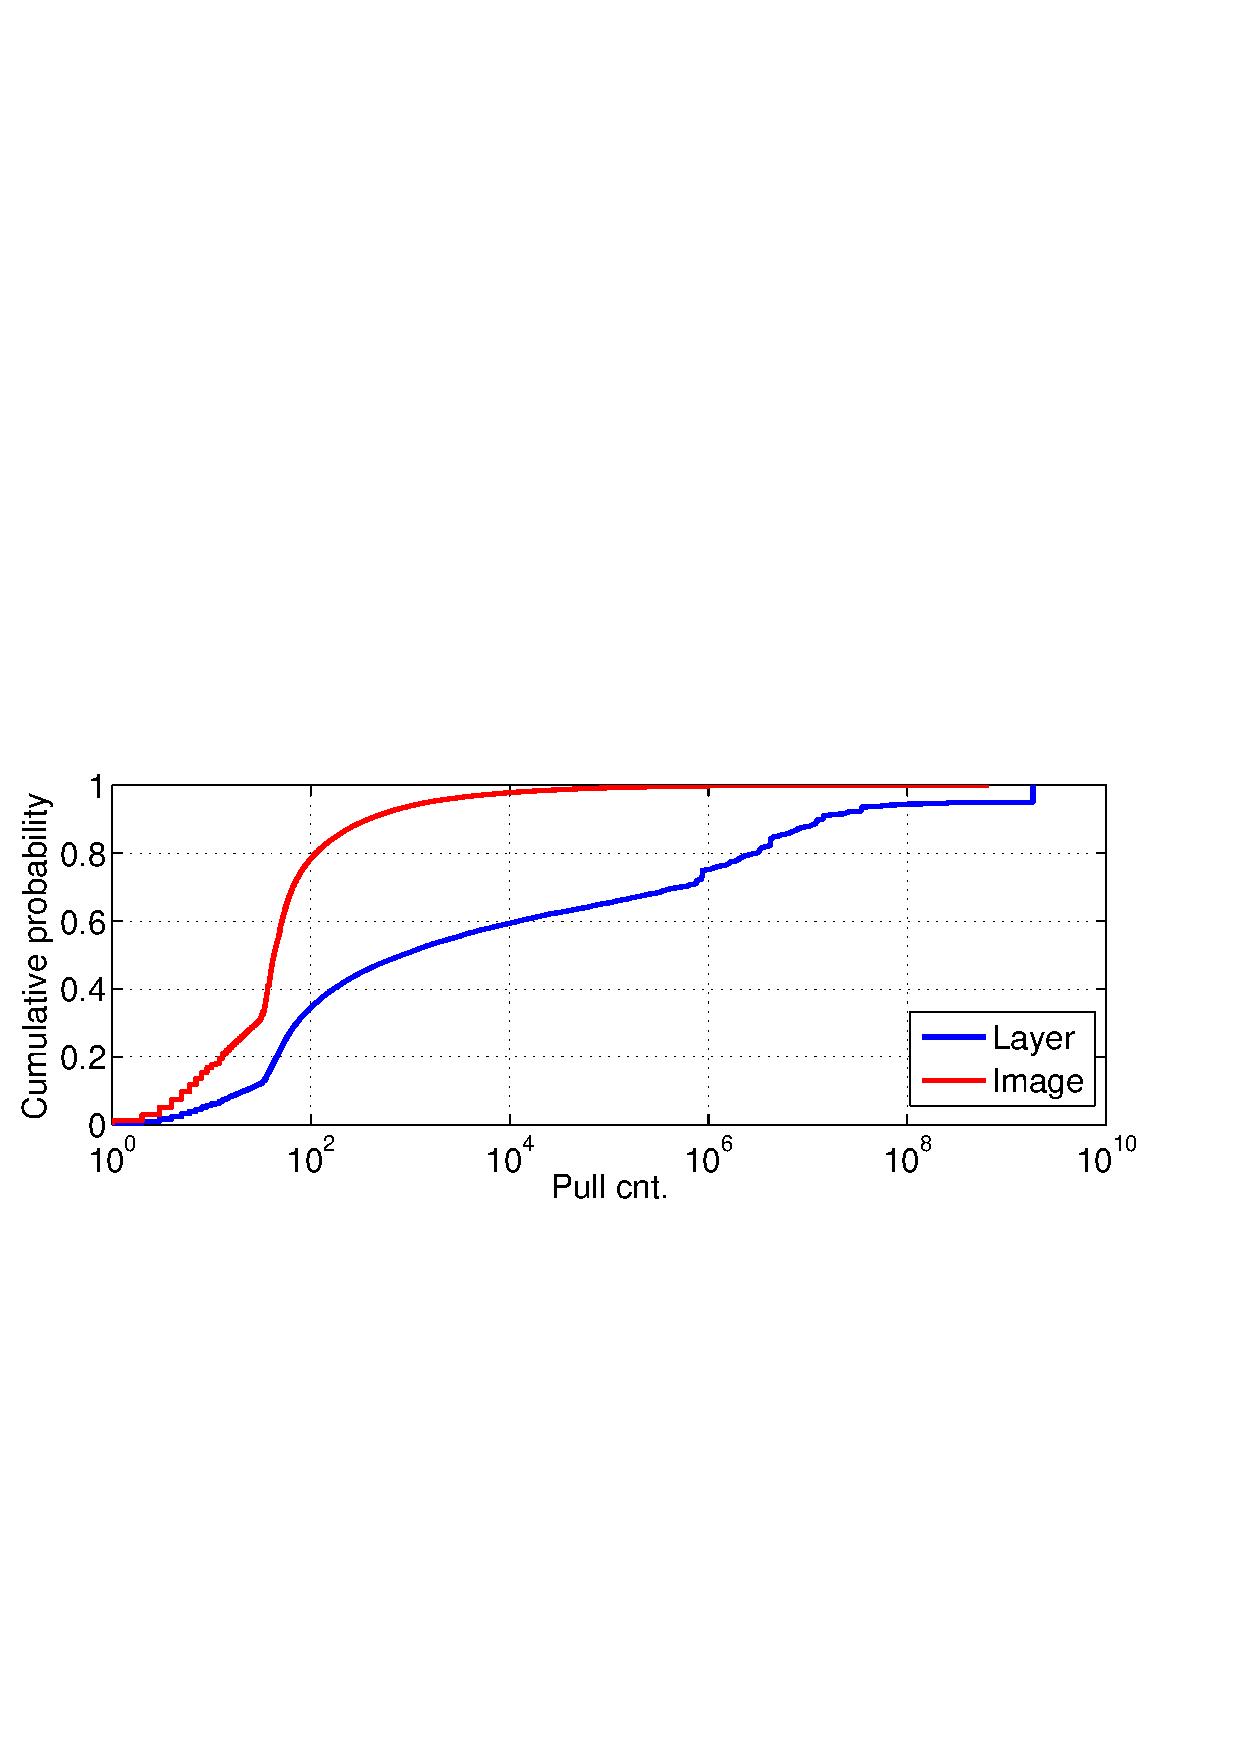
\includegraphics[width=0.23\textwidth]{graphs/pull_cnt.pdf}
	}
	\subfigure[Histogram of repositories by pull count]{\label{fig_pull_cnt_count}
		\includegraphics[width=0.22\textwidth]{graphs/count_pull_cnt.pdf}
	}
	\caption{Repository popularity distribution}
	\label{fig-pop}
\end{figure}

\paragraph{Image popularity}
%
We start by analyzing image popularity.
Figure~\ref{fig-pop} shows the repository popularity distribution on May 31st in
terms of the pull count of individual images.
%The x-axies show the pull count (i.e., total number of pulls) for repositories
%by May 31th with different ranges.  
The CDF in Figure~\ref{fig_pull_cnt_total} reveals a large degree of skew in image
pulls. In the median, images are only pulled 40 times while in the 90\% percentile we
see a pull count of 333. On the other hand, the largest pull count is more than 650 million
which is for the official \textit{nginx} repository. This is followed by
Google's \textit{cadvisor} (434 million pulls), \textit{redis} (264 million pulls),
\textit{ubuntu} (28 million pulls) and GliderLabs' \textit{registrator} (212 million pulls).


Looking at the pull frequencies for repositories (see Figure~\ref{fig_pull_cnt_count})
confirms the skewness. We see that 31,200 of repositories are only pulled between 0 and
2 times while 34,100 repositories are pulled between 3 to 5 times. What is interesting is
that there is a second peak around a pull count of 37 which does not fit a heavy-tailed
distribution. \lrcomment{Any explanation for this?}

%and 27,600 repositories are pulled
%~37 times, which are the two peaks shown in the figure.  Overall, repository
%frequency decreases with the pull count.

The skewness of two curves in figure~\ref{fig-pop} suggests that Docker hub is
a good fit for caching popular repositories or images to
reduce \textit{pull} latencies.

%%%%%%%%%%%%%%%%%%%%%%%%%%%%%%%%%%%%%%%%%%%%%%%%%%%%%%%%%%%%%%%%%%%%%

\paragraph{Image size distribution}
\label{sec:image-size}


\begin{figure}[!t]
	\centering
	\subfigure[CDF of images by size (GB)]{\label{fig_image_size_gb}
		\includegraphics[width=0.22\textwidth]{graphs/size.pdf}
	}
	\subfigure[CDF of images by size (MB)]{\label{fig_image_size_mb}
		\includegraphics[width=0.23\textwidth]{graphs/size_mb.pdf}
	}
	\caption{Image size distribution}
	\label{fig-image-size}
\end{figure}


\begin{figure}[!t]
	\centering
	\subfigure[CDF of layer count in images]{\label{fig_layer_cnt_less}
		\includegraphics[width=0.23\textwidth]{graphs/layer_cnt_less.pdf}
	}
	\subfigure[Histogram of layer count in images]{\label{fig_hist_layer_cnt}
		\includegraphics[width=0.213\textwidth]{graphs/hist_layer_cnt.pdf}
	}
	\caption{Layer count}
	\label{fig-layer-cnt}
\end{figure}

Similarly to layers, we also measure compressed image size
(CIS), \ie the sum of the sizes of the compressed image layers, and the sum of the
sizes of files contained in the image (FIS). Figure~\ref{fig_image_size_gb}
and~\ref{fig_image_size_mb} show the image size distributions at a coarse GB resolution
and a finer resolution only covering images less than 1.5 GB.

90\% of the images have an uncompressed size less than 1.3 GB while compressed images
are less than 0.48 GB. In the median, this decreases to 94MB and 17 MB respectively.
The largest uncompressed image is 498 GB which is a Ubuntu-based image.
Figure~\ref{fig-image-size} shows that the majority of uncompressed images in Docker Hub are
small which aligns with the Docker philosophy to package software and distribute
software in containers but include only its necessary dependencies.

%As shown in figure~\ref{fig_image_size_gb}, The CDF distribution of images for AIS and FIS are
%almost similar. 90\% of images have a less than 1.3GB decompressed size for either FIS or AIS,
%while 90\% of images can be compressed less than 0.48 GB. The largest AIS and FIS are ~498 GB
%while the largest CIS is only 202 GB.

%Figure~\ref{fig_image_size_mb} shows the cumulative image probability by image size in MBs.
%70\% of the images can be compressed less than 190 MB. And 70\% of the images have a less
%than 478 MB uncompressed size (i.e., AIS or FIS). Half of the images can be compressed less
%than ~17 MB. Half of the images are less than 46 MB in AIS format and 94 MB in FIS formats
%respectively.

%\paragraph{Compression rate distribution}
%
%\begin{figure}[!t]
	\centering
	\subfigure[CDF of images by compression ratio]{\label{fig_image_compression_ratio}
		\includegraphics[width=0.23\textwidth]{graphs/compression_ratio_less.pdf}
	}
	\subfigure[Histogram of images by compression ratio]{\label{fig_image_compression_ratio_less}
		\includegraphics[width=0.223\textwidth]{graphs/hist_compression_ratio.pdf}
	}
	\caption{Compression rate distribution}
	\label{fig-image-compression-ratio}
\end{figure}
%
%To understand compressibility, we again compute the FIS-to-CIS compression ratio
%
%%As discussed in~\ref{sec:image-size}, three kinds of image size are measured: AIS, CIS, and
%%FIS. Thus, we calculated two kinds of compression ratio: the ratio of AIS to CIS (AIS-to-CIS)
%%and the ratio of FIS to CIS (FIS-to-CIS).
%
%Figure~\ref{fig-image-compression-ratio} shows the cumulative image probability by compression
%ratio. Overall, we can see that AIS-to-CIS is greater than FIS-to-CIS. 90\% of images have a
%AIS-to-CIS less than ~4 while 90\% of images have a FIS-to-CIS less than 35. Half of the images
%have a compression ratio (both AIS-to-CIS and FIS-to-CIS) around 3. The maximum compression
%ratio are 512,930 and 1028 in FIS-CIS and AIS-CIS formats respectively.
%Figure~\ref{fig_image_compression_ratio_less} shows a histogram of image probability by
%compression ratio. 134,000 images' FIS-to-CISs are 3.5 and 90,000 images'AIS-to-CISs are 2.5,
%which are two peaks shown in the graph.
%
%Figure~\ref{fig-image-compression-ratio} suggests that Docker images has a great potential
%for compression to save space.

%%%%%%%%%%%%%%%%%%%%%%%%%%%%%%%%%%%%%%%%%%%%%%%%%%%%%%%%%%%%%%%%%%%%%


\paragraph{Layer count distribution}

As discussed in~\ref{sec-image-layers}, images consist of a set of layers.
It is important to understand the layer count of the images as previous
work found that the number of layers can impact the performance of
I/O operations~\cite{slacker}. Therefore, we count the number of layers
per image and plot the CDF (see Figure~\ref{fig-layer-cnt})
and layer count frequencies (see Figure~\ref{fig_hist_layer_cnt})for all
Docker Hub images.

The results show that 90\% of the images have less than 18 layers while
half of the images have less than 8 layers. 8 layers is also the most
frequent layer value with 51,300 images consisting of exactly 8 layers.
The maximum layer count is 120 in the \textit{cfgarden/120-layer-image}.
We also find that there are 7,060 images which only consist of a single layer.

\begin{figure}[!t]
	\centering
	\subfigure[CDF of layer by layer count]{\label{fig_repeate_layer}
		\includegraphics[width=0.23\textwidth]{graphs/repeate_layer.pdf}
	}
	\subfigure[Histogram of images by layer count in images]{\label{fig_hist_repeate_layer}
		\includegraphics[width=0.223\textwidth]{graphs/hist_repeate_layer.pdf}
	}
	\caption{Compression rate distribution}
	\label{fig-repeat-layer-cnt}
\end{figure}

%\paragraph{Repeat layer count distribution}

An interesting question is what is the sharing rate of layers across images.
We analyze all image manifests and count for each layer, how many times it
is referenced by an image. Figure~\ref{fig_repeate_layer} shows that around 90\%
of layers are only reference by a single image while 95\% are reference by not
more than 2 images.
%99\% of layers are shared among less than 25 images. 
%
Figure~\ref{fig_hist_repeate_layer} shows the absolute values, revealing that
almost 1.5 million images are only referenced once. While there is again a large
spectrum of reference counts, the maximum is 33,428, the vast majority of layers
is not shared. This hints that the layer-based approach to improve storage
efficiency is barely utilized and there is room for improvement in how images
are constructed.


%%%%%%%%%%%%%%%%%%%%%%%%%%%%%%%%%%%%%%%%%%%%%%%%%%%%%%%%%%%%%%%%%%%%%


\paragraph{Directory and file count distribution}

\begin{figure}[t]
	\centering
	\begin{minipage}{0.26\textwidth}
		\centering
		\includegraphics[width=1\textwidth]{graphs/dir.pdf}
		\caption{CDF of images by\newline directories}
		\label{fig-dir}
	\end{minipage}%
	\begin{minipage}{0.24\textwidth}
		\centering
		\includegraphics[width=1\textwidth]{graphs/file.pdf}
		\caption{CDF of images by files}
		\label{fig-file}
	\end{minipage}
\end{figure}

Lastly, we look at the directory (see Figure~\ref{fig-dir}) and file counts
(see Figure~\ref{fig-file}) in images to determine if deploying
images requires handling of large amounts of metadata. Looking at directories,
we see that 90\% of images have less than 7,344 directories while the median
is at 296. For files, 90\% of images have less than 64,780 files with a median
of 1,090.

This is consistent with with our analysis of layer-based file and directory counts
and the number of layers per image. Again, we conclude that most images
do not require an extensive amount of metadata when being deployed as file and
directory counts are low except for few outliers.

%Figure~\ref{fig-dir} shows the cumulative image probability by directories. 90\% of images
%have less than 7,344 directories. Half of images have less than 296 directories. The maximum
%is 1,168,160 while the minimum is 1. The average is 2,705. 

%Figure~\ref{fig-file} shows the cumulative image frequency by files. 90\% of images have
%less than 64,780 files. Half of images have less than 1,090 files. The maximum is 8,509,958
%while the minimum is 1. The average is 21,413.


\section{File-level deduplication analysis}
\label{sec:redundant_files}
%\nancomment{1. high repeat cnt type examples
%			2. use case for each type
%			3. analyze the others cluster, if have time}

%Based on the second-and third-level classification, we investigated the following two research questions: (1) What are the common redundant files?
%(2) Why there are so many redundant files? and present our investigation results.

%As discussed in Section~\ref{xxx}, analysis of compression ratio indicates that
%plenty of redundant data exists in individual layers and images. However, it's
%unknown how much redundant data is in Docker registry. 

In this section, we
investigate the potential for data deduplication in Docker registry. 
Since, layers are stored in gzip compressed format and layers are not
duplicated, we decompressed and unpacked all the layers, and conducted
deduplication analysis on the uncompressed dataset.
 
We adapt file-level deduplication strategy to find out whether
there are full file duplicates.%duplicates of source codes, scripts,  files, documents, etc.
File-level deduplication is a simple and efficient content-based deduplication
strategy, which can eliminate files whose full content is a duplicate of
another file. To find out how many full file duplicates in the dataset, we
calculated a digest of the complete file by using MD5 hash algorithm~\cite{xxx} and
presents file-level deduplication analysis results.
%A simple deduplication is to eliminate the replicates of full content of a
%file.  
%In this section, we investigate how many duplicate files are in layers, images, and registry in term of file count and capacity and present the results.
%\nancomment{will replace all graphs}
%\subsection{Deduplication ratio with layer-level content addressable store}
\label{sec:dedup_layerCAS}


\subsection{Data reduction analysis} 
\label{sec:dedup_ratio}

\paragraph{Layer sharing}

In its simplest implementation Docker would not support layer sharing.
%
Instead, every image would be a single flat archive.
%
In fact, some existing containerization frameworks
~\cite{singularity}~\cite{openvz} 
%
\VT{cite singularity and openvz}
%
\NZ{addressed}
%
\VT{No, not addressed, citation for singularity is still missing}
%
use flat images.
%
Our estimates show that without layer sharing Docker Hub dataset would grow
from 47TB to 85TB, implying \textbf{1.8$\times$} deduplication ratio provided
by the layer sharing technique.
 
We further computed for each layer, how many times it is referenced by images.
%
Figure~\ref{fig:ref_count} shows that around 90\% of layers are referenced by
only a single image, additional 5\% are referenced by 2 images, and less than
1\% of the layers are shared by more than 25 images.
%
Interestingly, there is one layer that is referenced by 184,171 images.  Our
analysis revealed that this is an empty layer. 
%
In addition, we found 7 layers that are referenced by 29,200 - 33,413 images.
They are mainly related to ubuntu 14.04.2, dpkg, apt, and cowsay. 
\NZ{Some layer tarfiles are not easy to describe. AND. these above layers are not 
	referred by official Ubuntu latest. Find an interesting thing: image name already
	tells what software packages it contains.} 
%
\VT{Explain the reason for empty layer.}
%
\VT{I feel we might need to talk about 2 more "most referenced" layers.}
\NZ{addressed}
%
\VT{Use \% instead of probability in all Figures (both  \# and labels).
We use \% in the text, so we MUST do it.}

\begin{figure}[t]
	\centering
		\begin{minipage}{0.2\textwidth}
			\centering
			\includegraphics[width=1\textwidth]{graphs/shared-cnt-cdf.pdf}
			\caption{CDF of layer reference count.}
			\label{fig:ref_count}
		\end{minipage}
	\begin{minipage}{0.22\textwidth}
		\centering
		\includegraphics[width=1\textwidth]{graphs/layer-size-cdf.pdf}
		\caption{CDF of compress. and uncompress. layer size.}
		\label{fig:layer-size-cdf}
	\end{minipage}%
\end{figure}
%%		\vcomment{Figures \ref{fig:layer-size-cdf} and \ref{fig:compress-ratio}
%have different sizes, looks not neat, please fix.}
%\begin{figure}
%	\centering
%	\includegraphics[width=0.21\textwidth]{graphs/shared-cnt-cdf.pdf}
%	\caption{CDF of layer reference count.
%	}
%	\label{fig:ref_count}
%\end{figure}
%
%+-----------------------------------------------------------------------+----------------+
%|layer_id                                                               |shared_image_cnt|
%+-----------------------------------------------------------------------+----------------+
%|sha256:a3ed95caeb02ffe68cdd9fd84406680ae93d633cb16422d00e8a7c22955b46d4|184171          | empty
%|sha256:e190868d63f8f8b85b026e53b5724c3c2a4548e1d642953442559cfa5f79b2c9|33413           | ubuntu 14.04.2 LTS. 
%|sha256:909cd34c6fd77d398af1d93e9d4f7f76104903f237be3d4db7b345a19631f291|33323           | dpkg
%|sha256:0b9bfabab7c119abe303f22a146ff78be4ab0abdc798b0a0e97e94e80238a7e8|33295           | apt
%|sha256:8eed3712d2cfd8c37b19d324452ba9cdb445933c04c9175c4e945b0d7241f1e3|31517           | cowsay
%|sha256:c57b6bcc83e3e88fb3748ea3f0cb13d77c4e2ffa7b9a8ded3d636f17d2d83759|31503           | cowsay 3.03 installasion package
%|sha256:8978f6879e2f86eb7a063e70f7d89feecde9950c40fc68f1f53d00b3c8ce9b52|31179           | same cowsay but different git info
%|sha256:00bf65475aba8f1077fa9629f088a5f531d645faeccb6acd7a8626c7d896a4c4|29200           | (looks like linux distribution)
%|sha256:386a066cd84a33a04d560c42bef66d1dd64ebfc76de78550e5fd0f8d57778bca|6103            |
%|sha256:3690ec4760f95690944da86dc4496148a63d85c9e3100669a318110092f6862f|4678            |
%|sha256:5c90d4a2d1a8dfffd05ff2dd659923f0ca2d843b5e45d030e17abbcd06a11b5b|4635            |
%|sha256:6d827a3ef358f4fa21ef8251f95492e667da826653fd43641cef5a877dc03a70|4496            |
%|sha256:627beaf3eaaff1c0bc3311d60fb933c17ad04fe377e1043d9593646d8ae3bfe1|4025            |
%|sha256:e110a4a1794126ef308a49f2d65785af2f25538f06700721aad8283b81fdfa58|4001            |
%|sha256:357ea8c3d80bc25792e010facfc98aee5972ebc47e290eb0d5aea3671a901cab|3952            |
%|sha256:6a5a5368e0c2d3e5909184fa28ddfd56072e7ff3ee9a945876f7eee5896ef5bb|3927            |
%|sha256:75ea8418708338e40dce9179cfe97fd116831f1601be50fef48ea6011653c986|3895            |
%|sha256:75a822cd7888e394c49828b951061402d31745f596b1f502758570f2d0ee79e2|3793            |
%|sha256:f94adccdbb9cec09b3e64ec31aab2b07cbc020fe8f9151418ca6b7ede22273c0|3717            |
%|sha256:693502eb7dfbc6b94964ae66ebc72d3e32facd981c72995b09794f1e87bac184|3701            |
%+-----------------------------------------------------------------------+----------------+

\paragraph{Compression}
%
Figure~\ref{fig:layer-size-cdf} presents compressed and uncompressed layer size
distributions.
%
We find that 50\% of the layers are less than 1MB and 90\% of the layers are
less than 64MB in compressed format.
%
If uncompressed, 50\% of the layers are smaller than 2 MB and 90\% of the
layers are smaller than 170MB.
%
Moreover, the total compressed layer dataset grows from 47~TB to 167~TB after decompression, resulting in \textbf{3.6$\times$} compression ratio.

\paragraph{File-level deduplication}
%
Next, we calculate deduplication ratio in terms of file count and capacity for
the complete uncompressed dataset.
%
After removing redundant files, there are only 3.17\% of files left that occupy
23.92~TB, resulting in deduplication ratios of \textbf{31.55$\times$} and
\textbf{6.99$\times$} in terms of file count and capacity, respectively.
%
\begin{figure} \centering
	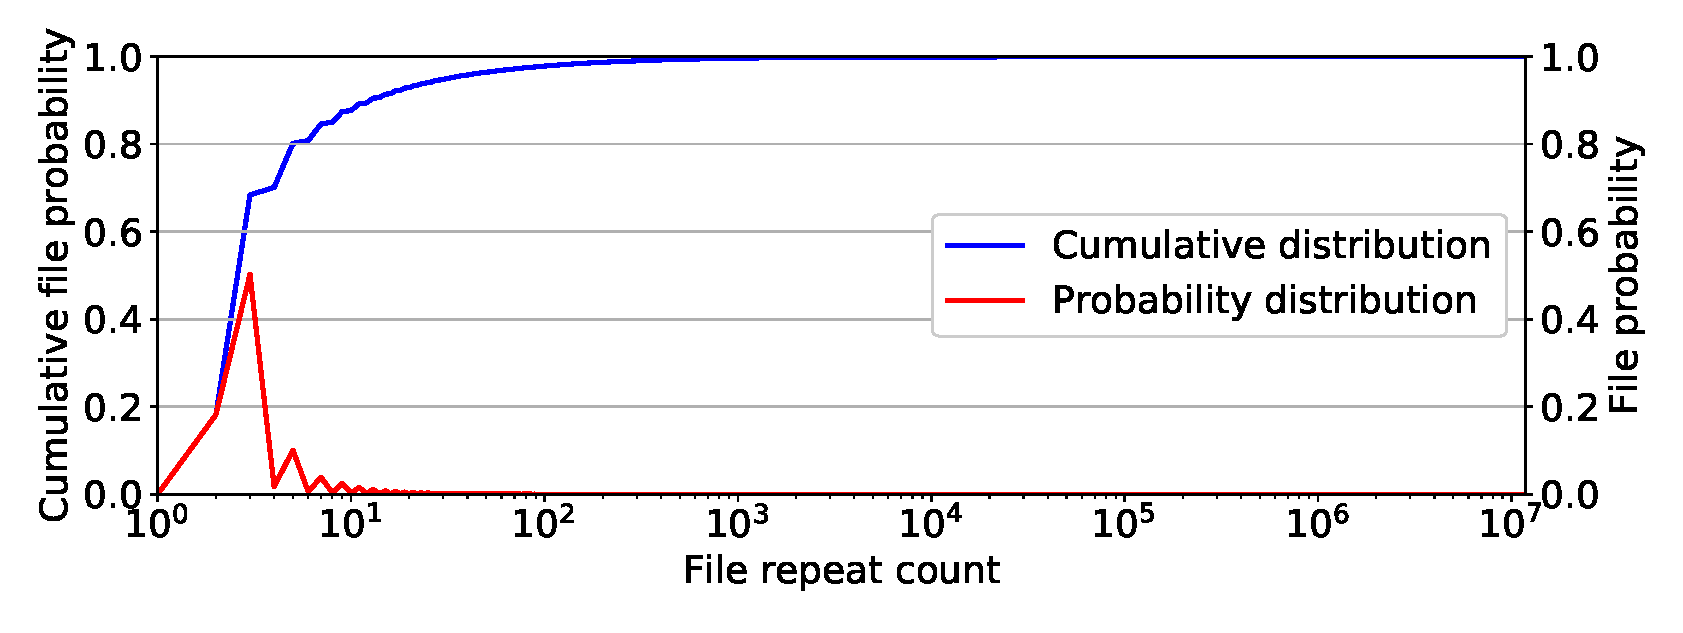
\includegraphics[width=0.45\textwidth]{graphs/File_repeat_count.eps}
	\caption{File repeat count distribution.
	%
	\VT{No need for Y2}
	%
	\VT{Still need to use \% on the axis}
	%
	} \label{fig:file-repeat-cnt}
\end{figure}

%
We further analyzed the repeat count for every file.
%
Figure~\ref{fig:file-repeat-cnt} shows the distributions of file repeat count.  
%
We see that over 99.42\% of files have more than one copy.
%
Around 50\% of files have exactly 4 copies and 90\% of files have 10 or less
copies. 
%
The file that has the maximum repeat count 53,654,306---is an empty file.
%
\VT{Do we know anything about those empty files}.
%

%
\VT{I believe we need to talk about over frequent files. Maybe in the text
section.}.

\subsection{Deduplication by file types}

\begin{figure} 
	\centering
	\includegraphics[width=0.45\textwidth]{graphs/dedup-overall} 
	\caption{Deduplication ratio for seven file classes---EOL, archival, document, source code, database, scripts, images---and other files
%
\VT{Can we stretch X axis to column width to have more space for X-axis labels?}
%
\VT{Explain what blue and red bars mean here, as well as dots. Explain
if dedup ratio is in terms of capacity or file counts.}
%
} 
	\label{fig:dedup-overall} 
\end{figure}


To understand the sources of high data redundancy among Docker images, we
investigate deduplication for common file types.
%
We identify 133 file types (e.g., JPG, C/C++, and Java files)
using the file type library~\cite{pymagic} and then group file types into 7
classes by their high-level use cases:
%
1)~executable, object, and library files (EOL) (such as .o or .pyc)
%
%\VT{Maybe call them ``Exec.`` instead on the graph and everywhere?}
%
2)~archival (such as .gz or .tar),
%
2)~documents (such as .txt or .tex),
%
4)~source code (such as .c or .java),
%
5)~scripts (such as .py or .js),
%
6)~images (such as .png or .eps), and
%
7)~database files (such as .sqlite or .frm). 
%
These classes cover about 88\% of the whole dataset (by capacity);
we group the remaining 12\% in the Others class.
%

Figure~\ref{fig:dedup-overall} illustrates the deduplication results for these
classes.
%
The overall deduplication ratio is \textbf{6.9$\times$} and 4 type classes
have a comparable ratio (indicated by the dots in the figure).
%
For example, the deduplication ratio for EOL files is \textbf{7.1$\times$}.
%
However, for the other 3 type classes, the
deduplication ratio is significantly
higher---\textbf{31.25$\times$} for source code,
\textbf{50$\times$} for scripts, and \textbf{12.5$\times$} for documents.
%
This indicates that users are prone to frequently replicate
source code, scripts, and documents in their images.
%
%Moreover, the source code and script duplicates generate additional executables
%and object files that are identical.

We found that redundant C/C++ source code takes up over 77\% of the capacity
occupied by source code.
%
Looking closer we found that, for example, Google Test~\cite{googletest}---a
cross-platform C++ test framework available on GitHub~\cite{github}---is
frequently replicated.
%
Interestingly, we found there are multiple Docker repositories related to
Google Test while there is no official repository for Google Test.
%
We suspect that many developers replicate open source code from external public
repositories, such as GitHub, and store it in container images but do not
specifically encapsulate it in a separate layer.
%
This would also explain the shared source code across different images.
%
%\VT{give few more example in addition ot Google Test}\NZ{addressed}
% 
In addition to Google Test, we also found source code of
go-ethereum~\cite{go-ethereum}, Android Native Development Kit (NDK)~\cite{NDK},
xnu-chroot-environment~\cite{xnu-chroot-environment} among others.
%
%Docker Hub allows developers to automatically build images from
%source code in external public repositories and automatically push the built
%image to their Docker repositories. 
%%https://github.com/ethereum/go-ethereum
%https://github.com/postgres/postgres
%We believe that 
%many developers would replicate
%%more 
%open source codes
%%may be replicated 
%into different images stored in Docker Hub registry.
%
%\VT{I don't understand the last sentence. ``more'' than what?.. And who can 
%replicate? don't use passive voice to make it clear.
%Also, last sentence is too long, please, split.}
%\NZ{commented}
%\VT{not yet ;)}
%
%\textit{To eliminate redundant open source codes in Docker registry in the
%future, we suggest that Docker Hub creates offical images for popular
%open source codebases so developers can directly pull the image as a
%read-only layer}.

Next, we observe that redundant EOL and archival files occupy over half of the
total dataset
capacity (51.4\%). 
%\LR{capacity of what?}\NZ{addressed}.
%
%To understand why there are so many redundant archival files, 
%we manually
%inspected them and found that many archival files contain source codes.
%
%\VT{``many'' is vague}\NZ{addressed}
Additionally, we analyze the top-5 most frequent archival files.
We found that \texttt{NEWS.Debian.gz}, which stores news
about package changes has 521,611 copies.
Additionally, \texttt{pwunconv.8.gz}, which is used to create passwords
has 358,374 copies.
There are two files that have around 86,733 copies respectively:
\texttt{ubuntu\_dists\_trusty\_universe\_Sources.gz} and
\texttt{ubuntu\_dists\_trusty\_universe\_binary-\\amd64\_Packages.gz}, which
contains the name, version, size, the description, and the dependencies of each package.
%
The last file, \texttt{gcc.log.xz} has 13,384 copies and belongs to the GNU C++ compiler.
%
%For example, we found a highly redundant zip file called
%android-ndk-r12b.zip~\cite{NDK}.
%
%\VT{how many instances of this file were there?}\NZ{addressed}
%
%It packages Android Native Development Kit (NDK) that allows Android
%application developers to include native code in their Android application
%packages, compiled as JNI shared libraries~\cite{NDK}.
%
%\VT{So, Android developers use Docker?..}\NZ{addressed}
% shared-mime-info 24415
%This is mainly because EOL and archival file sizes are bigger than other type
%group.
%
 
%Database related files have the lowest deduplication ratio (\textbf{4.2$\times$}),
%which contributes little to the overall savings.

%All common file types have a high deduplication ratio.  Especially, EOL and
%archival files contribute a lot to the overall savings.
%
%Also, developers are likely to reuse code rather than create their own.
%
%\DIM{Ffrom the data we see there is high source code dedup, but this might be
%too much of a generic statement based on this data.}

%We see that 43.15\% of redundant files are documents, 
%%
%Documents have the
%largest number of redundant files (), indicating that users replicate more
%documents than other clusters. While the redundant document files only consume
%14.54\% (20.87 TB) of storage space, indicating that the size of redundant
%document files are small (10.2 KB on average). In comparison, 13.38\% and
%10.23\% of files are EOL files and source codes, which take up over 3.66\%
%(5.3 TB) and 36.85\% (52.9 TB) of redundant storage space, indicating that
%users replicate source codes and create big identical EOF files (108.6 KB on
%average).
%
%Archival files and scripts have almost similarly number of redundant files,
%8.53\% for archival and 8.69\% for scripts. However, archival cluster consumes
%more storage space than that of scripts (32.9 TB for archival and 3.9 TB for
%scripts) since archival file size (81 KB on avg.) is inherently higher than
%script size (9.4 KB on avg.).
%
%We found that 4.15\% of redundant files are image files and 0.09\% of
%redundant files are relevant to database, which takes 2.1 TB and 3.9 GB
%storage space respectively. There are 10.17\% (21.2 TB) of redundant files in
%\textit{Other} cluster which mainly contains binary data (9.76), GNU message
%catalog (3.37 TB), font related type (3.02 TB), git pack files (1.9 TB), etc. 
%
%\textit{ Finding 1: 13.38\% and 10.23\% of redundant files are source codes
%and EOL files, which take up over 3.66\% (5.3 TB) and 36.85\% (52.9 TB) of
%redundant storage space, indicating that users are more prone to replicate
%source codes and create identical big EOF files, while 43.15\% and 8.53\% of
%redundant files are documents and archival files, which account for 14.54\%
%(20.87 TB) and 22.93\% (32.9 TB) of redundant storage space, indicating users
%replicates more documents and archival files compare to other clusters.}


%
%\begin{figure} 
%	\centering
%	\includegraphics[width=0.35\textwidth]{graphs/dedup-eol} 
%	\caption{Deduplication results for EOL files: ELF, intermediate representation, PE32/PE32+ files, Debian/RPM binary packages, 	Libraries, COFF files.} 
%	\label{fig:dedup-eol}
%\end{figure}
%
%\paragraph{Executable, object code, and libraries (EOL)} We further calculated
%the deduplication ratio for specific file types in each common type group. 
%%
%We
%started from EOL group since it occupies the most capacity and contributes a
%lot to the overall savings after deduplication. 
%%
%Figure~\ref{fig:dedup-eol} shows the deduplication results for EOL files.  
%%
%We
%see that ELF files, intermediate representations, and PE files have the highest
%deduplication ratio (around 87\%). 
%%
%Especially, the redundant ELF files occupy
%the most capacity (73.4\%). 
%%\nancomment{replace MS exec with PE files}
%Libraries and COFF files have the lowest deduplication ratio of 53.5\% and 61\%
%respectively.
%
%We also calculated the deduplication ratio for each intermediate representation
%and libraries. 
%%
%We found that all the intermediate representations have a very
%higher deduplication ratio (greater than 77\%). 
%%
%Especially, the redundant
%Python byte-compiled codes take up to 67\% of capacity occupied by intermediate
%representations. 
%%
%Although overall library's deduplication is lower, we found
%that GUN C/C++ library and Palm OS dynamic library have a higher deduplication
%ratio over 90\%.
%
%\textit{Finding 4: ELF files have the highest deduplication ratio among all EOL
%files and contribute most to the overall savings. Python byte-compiled codes
%have the highest deduplication ratio and also achieve a better capacity savings
%after dedupliation compared with other intermediate representations. Most
%libraries have the lowest deduplication ratio among all EOL files.}
%%
%%%As shown in , intermediate compiled files have the largest number of
%%redundant copies (333,261,220, 63.7\%), which only take up to 5.3\% (2.8TB) of
%%EOL redundant storage space, indicating that users creates more small
%%redundant intermediate compiled files. Among all the intermediate compiled
%%files, python byte-compiled files have the largest number of redundant copies
%%(64.1\%, 213,753,591), which account for 79.4\% (2.2TB) of EOL redundant
%%storage space as shown in Figure~\ref{fig:type-compiled}.  % %We found that
%%there are various redundant intermediate compiled files in layers in addition
%%to Python byte-compiled, such as Erlang beam files, Xemacs/emacs compiled
%%files, compiled Java class, Mach-o fat files, Guile object bytecode, and llvm
%%bitcode files. We see that 21.6\% (71,830,155) and 10.12\% (33,740,399) of
%%redundant intermediate compiled files are terminfo compiled and compiled java
%%class files, which consume 76.4 GB and 104.4 GB storage space.   
%%
%%%ELF files have the largest redundant capacity %A large executable group is
%%ELF file type, which consists of ELF 64/32-bit LSB relocatable, shared object,
%%executable, core file, processor-specific for x86-64, MIPS, %ARM, Intel 80386,
%%etc. architectures.  %Another executable group contains VAX COFF executable,
%%PE32/PE32+ executable for Windows, and 386 pure executable, VMS Alpha, etc.
%%%\% of files are script executable, which contains python, shell, etc.  %\% of
%%files are RPM, Debian bin
%%
%%%\begin{figure} %	\centering %
%%\includegraphics[width=0.5\textwidth]{graphs/type-exec-cap} %
%%\caption{\nancomment{Deduplication results for EOL files}.  %	} %
%%\label{fig:type-eol} %\end{figure}
%%
%%%Finding 2: 31.4\% (164,059,690) and 63.7\% (333,261,220) of EOL files are ELF
%%files and intermediate compiled files, which take up over 85.7\% (45.3TB) and
%%5.3\% (2.8TB) of redundant storage capacity, indicating that users replicate
%%or create more identical ELF files and intermediate compiled files. 64.1\%
%%(213,753,591) of intermediate compiled files are Python byte-compiled files,
%%which take up to 79.4\% (2.2TB) of redundant storage space, indicating that
%%users compiled more Python scripts (similar to Finding 2.)
%%
%\paragraph{Source code (SC.)}
%%
%%%Finding 3: 80.2\% (548,507,865) of source codes are C/C++ source, which take
%%up to 79.7\% (4.2TB) of redundant storage space, indicating that users are
%%more prone to duplicate C/C++ codes, which results in more ELF file replicas.
%%%The last group contains
%%
%\begin{figure} 
%	\centering
%	\includegraphics[width=0.35\textwidth]{graphs/dedup-sc} 
%	\caption{Deduplication results for source codes: C/C++ source, Perl5 module source, ruby module
%		source, pascal program, fortran program, Applesoft Basic program, Lisp/scheme
%		program, and other source codes.  } 
%	\label{fig:dedup-sc} 
%\end{figure}
%
%As discussed, Docker developers are more prone to replicate codes. 
%%
%To find out
%which kind of source codes are replicated frequently, we conducted
%deduplication on 7 common source codes as shown in Figure~\ref{fig:dedup-sc}.
%
%We see that all the source codes have a high deduplication ratio over 90\%
%except Lisp/scheme program. 
%%
%Especially, the redundant C/C++ source codes take
%up over 77\% of capacity occupied by source codes. 
%%
%To find out why there are so
%many C/C++ source codes, we inspect the C/C++ source codes and find a
%frequently replicated C/C++ source code called Google Test~\cite{googletest}, which is
%a cross-platform C++ test framework and available in GitHub~\cite{github}.
%%
%Interestingly, we found there are plenty of repositories related to Google Test
%while there is no official repository for Google Test. 
%%
%We suspect that many
%developers replicate open source code from external public repositories, such
%as GitHub, and store them in containers. 
%%
%This would also explain why there are
%so many shared source codes across different images. 
%%
%Docker Hub
%allows developer to automatically build images from source code in external
%public repositories and automatically push the built image to their Docker
%repositories. Thus we believe that more open source code would be replicated into
%different images stored in Docker Hub registry. 
%%
%\textit{To eliminate redundant
%open source codes in Docker registry in the future, we suggest that Docker Hub
%can create more offical images for popular open source codes so that developers
%can directly pull the image as a read-only layer. }
%
%\textit{Finding 5: C/C++ source codes have a high redundant ratio and
%contribute a lot to the overall savings. Many redundant source codes shared
%cross images are replicated or automatically build from external public
%repositories. To eliminate redundant source codes in Docker registry, we
%suggest to create more official images for these open source codes and convince
%developers to pull them from registry.}
%%
%%%\nancomment{found some libc++ source code here, did not put them into
%%libraries.} % shows the redundant file count and storage capacity distribution
%%for source code. C/C++ source codes have the largest number of redundant
%%files. 80.2\% (548,507,865) of source codes are C/C++ source, which take up to
%%79.7\% (4.2TB) of redundant storage space, indicating that users are more
%%prone to duplicate C/C++ codes, which results in more ELF file replicas.
%%
%%%We also found other source codes, such as Perl5 module source code (9.5\%),
%%ruby module source code (7.6\%), assembler source code (1.1\%), pascal source
%%(0.7\%), fortran program code (0.01\%), applesoft basic source code, and
%%Lisp/scheme source code (0.17\%).
%%
%%%\begin{figure} %	\centering %
%%\includegraphics[width=0.5\textwidth]{graphs/type-lang-cap} %
%%\caption{Redundant data vs. unique data for source code files.  %	} %
%%\label{fig:type-source} %\end{figure}
%%
%%%Figure~\ref{fig:type-lib} shows the redundant library distribution. We see
%%that Gcc precompiled header files have the lowest number of redundant library
%%files (20.3\%), but they take up to 0.93 TB. Almost 86.4\% of redundant
%%library files are Palm libraries, which only take up to 7.2GB space,
%%indicating that gcc compiled header files are much bigger than other
%%libraries.  % %We also found there are different libraries used in layers,
%%such as netcdf library, Ocaml lib., mach-o lib.
%%
%%%Figure~\ref{fig-elf} %\subsection{Lib} % %library files contains libtool
%%library file, OCaml native library, MIT scheme, Mach-O library, OCaml library,
%%Palm OS dynamic library data, Microsoft c/c++ library.current ar archive
%%random library, and other library.
%%%%libtool\|OCaml\|Palm\|MIT\|microsoft\|current ar archive random
%%library\|mach-o\|rpm\|gzip %\subsection{Source code}
%%
%\paragraph{Scripts(Scr.)}
%%%Finding 2: 53.6\% (238,353,674) of redundant scripts are Python scripts,
%%which take up over 2.6TB storage space, indicating that users are more prone
%%to replicate Python scripts compare to other scripts.
%%
%%%\begin{figure} %	\centering %
%%\includegraphics[width=0.5\textwidth]{graphs/type-script-cap} %
%%\caption{Redundant data vs. unique data for scripts.  %	} %
%%\label{fig:type-script} %\end{figure}
%%
%
%\begin{figure} 
%	\centering
%	\includegraphics[width=0.45\textwidth]{graphs/dedup-scrp}
%	\caption{Deduplication results for scripts: python, AWK, ruby, perl, PHP, makefile, M4 macro processor, node, Tcl, bash and other scripts.}
%	\label{fig:dedup-scrp} 
%\end{figure}
%
%Similar to source codes, we present the deduplication ratio for scripts as
%shown in Figure~\ref{fig:dedup-scrp}.  
%%
%We see that most of the scripts have a
%high deduplication ratio over 95\%. 
%%
%Especially, the redundant Python scripts
%take up over 65\% of capacity occupied by scripts. 
%
%We inspect the Python scripts and found a frequently replicated Python scripts
%called kraken-tools~\cite{krakentools}, which is a tool for managing system
%requirements for kraken-lib~\cite{krakenlib}. 
%%
%kraken-lib is an orchestration and
%cluster-level management system for Kubernetes~\cite{kubernetes}.
%%% a tool for  for Kubernetes cluster.  %kraken-lib %Kubernetes is an open
%%source platform that automates Linux container operations 
%%
%Although kraken-tools seems like an Docker image repository, it is maintained
%in GitHub rather than Docker registry. 
%%
%Interestingly, kraken-lib does not have
%a official repository in Docker Hub but it has a public repository in QUAY
%registry~\cite{quay}.  
%%
%\textit{Similar to source codes, we suggest to create
%more official images in registry for some popular public scripts %, especially
%containerized applications and convince developers to pull them from registry
%as a read-only layer to reduce redundant scripts in registry.}
%
%\textit{Finding 6: Scripts have a very high deduplication ratio. Especially,
%redundant Python scripts contribute a lot to the overall savings. Many
%redundant scripts are replicated from external public repositories such as
%GitHub.  we suggest to create more official images for these public scripts and
%convince developers to pull them from registry.}
%%% shows the redundant scripts distribution. Python script has the largest
%%number of redundant scripts (238353674, 53.6\%), which take up to 2.6TB
%%storage space, indicating that users are more prone to replicate Python
%%scripts compare to other scripts.  %%This finding also explains that why
%%python byte compiled files takes the largest proportion of intermediate % %We
%%find that users use different scripts in the images.  %For example, 20\%,
%%9.7\% and 4.4\% of scripts are bash/shell scripts, ruby scripts, and awk
%%scripts. Other scripts such as perl script (4.2\%), php script(3.9\%),
%%makefile script(1.3\%), and M4 macro processor script(0.7\%) are also used.
%%
%\paragraph{Documents(Doc.)}
%%%Finding 3: 79.7\%, 5.2\%, and 12.4\% of redundant documents are ASCII text,
%%UTF-8/16 text, and HTML/XML/XHTML, which take up over 11TB, 3.4TB, and 3.9TB
%%redundant storage, indicating that users replicate more ASCII text, UTF-8/16
%%text, and HTML/XML/XHTML compare to other documents.
%%
%\begin{figure} 
%	\centering
%	\includegraphics[width=0.35\textwidth]{graphs/dedup-doc} \caption{Deduplication
%	results for documents: ASCII, UTF, ISO-8859, HTML/XML/XHTML, PDF, LaTex
%	documents, Composite document files, and others.} 
%	\label{fig:dedup-doc}
%\end{figure}
%
%Next, we present the deduplication results for different documents as shown in
%Figure~\ref{fig:dedup-doc}.  
%%
%We see that all the documents have a very high
%deduplication ratio of 84\% or higher.  
%%
%Especially, redundant raw text files
%and HTML/XML/XHTML documents take up over 48\% and 17\% of capacity occupied by
%documents. 
%%
%To understand why there are so many document duplicates, we inspect
%raw text files and HTML/XML/XHTML documents respectively. 
%%
%First, we found that
%a large amount of redundant raw text files are input data for testing source
%codes and they are replicated along with source code or script projects from
%external public repositories.  
%%
%For example, scipy~\cite{scipy}, a
%metamathematical software, is replicated from GitHub and stored in different
%images, which contains over 30 raw text files for testing purpose.
%
%Second, after inspected HTML/XML/XHTML documents, we found plenty
%HTML/XML/XHTML documents serves as readme, manual, or license. 
%%
%For example, we
%found plenty redundant HTML documents related to gnome-vfs-doc~\cite{gnome-vfs-doc},
%which are documentation for GNOME virtual filesystem subsystem available
%online~\cite{gvfs}.
%
%\textit{Finding 7: Documents have a very high redundant ratio. Majority
%redundant documents are raw text files and HTML/XML/XHTML documents. They are
%replicated along with source code or script projects and serves as input data
%for testing or informative documents.}
%%
%%%\begin{figure} %	\centering %
%%\includegraphics[width=0.5\textwidth]{graphs/type-utili-cap} %
%%\caption{Redundant data vs. unique data for documents.  %	} %
%%\label{fig:type-doc} %\end{figure}
%%
%%%https://pkgs.alpinelinux.org/contents?branch=edge&name=gnome-vfs-doc&arch=x86_64&repo=main
%%% presents redundant document distribution. We first group documents into two
%%categories: non-text documents and raw text documents.  %We see that ASCII
%%text files have the largest number of redundant document files (1,758,299,693,
%%79.7\%), which take up to 11TB storage space, indicating that users replicate
%%more ASCII text.  %12.4\% of the redundant documents are HTML/XML/XHTML
%%documents, which take up to 3.9 TB storage space, indicating users also
%%replicate HTML/XML/XHTML documents in images.  % %In addition to ASCII text,
%%5.2\% of redundant documents are UTF-8/16 unicode text, which take up 3.4 TB
%%storage space.  %Various documents are replicated in images, such as PS/PDF
%%documents (0.9\%), LaTex files (1.1\%) and Composite documents (0.01\%)
%%
%%%79.7\%, 5.2\%, and 12.4\% of redundant documents are ASCII text, UTF-8/16
%%text, and HTML/XML/XHTML, which take up over 11TB, 3.4TB, and 3.9TB redundant
%%storage, indicating that users replicate more ASCII text, UTF-8/16 text, and
%%HTML/XML/XHTML compare to other documents.  %type-utili-cap %type-script-cap
%%
%\paragraph{Databases (DB.)}
%%
%\begin{figure} 
%	\centering
%	\includegraphics[width=0.4\textwidth]{graphs/dedup-db} \caption{Deduplication
%	results for database related files.  } 
%	\label{fig:dedup-db} 
%\end{figure}
%
%As discussed, Database related files have the lowest deduplication ratio at
%file-level. 
%%
%It makes sense because it's unusual for different users to create
%large amount of identical database files. 
%%
%Figure~\ref{fig:dedup-db} shows the
%deduplication ratio for different types of databases. 
%%
%We see that SQLite
%database files have the largest deduplication ratio of 87\% and could be
%deduplicated for saving up to half of the capacity. 
%%
%To find out why there are
%so many redundant SQLite files, we inspected SQLite files manually and found
%majority of redundant SQLite files are created by Yum~\cite{yum} for
%maintaining a list of well-know repositories.
%
%\textit{Finding 8: Databases have a low deduplication ratio. But SQLite files
%have the largest amount of redundant files and contribute a lot for saving
%capacity. The redundant SQLite files are mainly for saving identical list of
%repositories.}
%%
%%%primary_db.sqlite
%%
%%%Finding 4: 28.7\%, 30.9\%, and 11.9\% of redundant database files are
%%Berkeley DB, Mysql, and Dbase related files, which only take up over 1.1 TB,
%%26 GB, and 47.2 GB redundant storage, indicating that users replicate a lot
%%small database files related to Mysql and Berkeley DB. While there are only
%%7.3\% of SQLite files, which take up over 2.6TB storage space, indicating
%%SQLite files are much bigger than others.  % %Figure~\ref{fig:type-db}
%%presents database related redundant files. 30.9\% of redundant database
%%related files are related to MySQL, which only take up to 26GB storage space
%%while SQLite database related redundant files which only take up 7.3\% of
%%redundant database related files consume 2.56 TB storage space, indicating
%%users replicate more MySQL related files and bigger SQLite database related
%%files. %MySQL related files contains mysql table definitation files, mysql
%%misam index files, and mysql misam compressed data.  %Moreover, we also find
%%different redundant database related files are replicated in Docker images.
%%For example, 28.7\%, 11.86\%, and 5.57\% of redundant database files are
%%Berkeley DB, Dbase, and NDBM related files, which take up over 1.1 TB, 47.2
%%GB, and 7.7 GB redundant storage, indicating that users replicate database
%%files, especially, SQLite and Berkeley DB.  %While there are only 7.3\% of
%%SQLite files, which take up over 2.6TB storage space, indicating SQLite files
%%are much bigger than others.
%%
%%
%%%\begin{figure*}[t] %	\centering %	\begin{minipage}{0.35\textwidth} %
%%\centering %
%%\includegraphics[width=1\textwidth]{graphs/type-db-cap.pdf} %
%%\caption{Redundant data vs. unique data for database related files} %
%%\label{fig:type-db} %	\end{minipage}% %
%%\begin{minipage}{0.278\textwidth} %		\centering %
%%\includegraphics[width=1\textwidth]{graphs/type-tar-type} %
%%\caption{Redundant data vs. unique data for archival files} %
%%\label{fig:type-arch} %	\end{minipage} %
%%\begin{minipage}{0.28\textwidth} %		\centering %
%%\includegraphics[width=1\textwidth]{graphs/type-image-cap} %
%%\caption{Redundant data vs. unique data for image files} %
%%\label{fig:type-img} %	\end{minipage} %\end{figure*}
%%
%%\paragraph{Archival (Arch.)}
%%
%%Figure~\ref{fig:type-arch} shows the deduplication ratio for each common
%%archival type.  We see that most of archival files have a high deduplication
%%over 80\% except tar archival files. Especially, Zip/Gzip files contribute to
%%most capacity savings after deduplication (62\%).  To understand why there are
%%so many redundant Zip/Gzip files, we manually inspected redundant Zip/Gzip
%%files and found that most of zip/Gzip files packages open source codes.  For
%%example, we found a redundant zip files called android-ndk-r12b.zip. It
%%packages the open source code--Android Native Development Kit (NDK)--that
%%allows Android application developers to include native code in their Android
%%application packages, compiled as JNI shared libraries~\cite{xxx}.
%%android-ndk-r12b.zip is available for downloading from GitHub. 
%%
%%\textit{Finding 9: Archival files have a high deduplication ratio. Majority of
%%Zip/Gzip files packages open source codes that are available online. We
%%suggest developers to remove the redundant archival files after unpacking to
%%reduce image size and save space.}
%%
%%%Finding 4: 89.5\% and 7.0\% of redundant archival files are Gzip files and
%%Zip files, which take up over 8.4 TB and 15.2 TB storage space, indicating
%%that users replicate more Gzip files and Zip files are much bigger than Gzip
%%files.  % % redundant archival file distribution. Gzip files have the largest
%%number of redundant archival files (89.5\%), which take up to 8TB storage
%%space, indicating that users replicate more Gzip compressed files. Although
%%Zip files only take 7.00\% of redundant archival files, they consume 15.5 TB
%%storage space since they are much bigger than Gzip files.  % %We found other
%%different kinds of archive files, such as XZ (0.42\%), Bzip2(0.96\%), and Tar
%%files(0.36\%).
%%
%\paragraph{Images (Img.)}
%
%\begin{figure} \centering
%\includegraphics[width=0.35\textwidth]{graphs/dedup-img} \caption{Deduplication
%results for image files.  } \label{fig:dedup-img} \end{figure}
%
%Last, we present the redundant ratio for image files as shown in
%Figure~\ref{fig:dedup-img}.  We see that most of image files have a high
%deduplication ratio over 80\% except TIFF image files and TIFF image files.
%Especially, PNG images contributes to almost half of capacity savings after
%deduplication.  To understand why there are so many redundant image files, we
%inspected redundant PNG images and found plenty of PNG images are logo, icons,
%wallpapers, and images for testing.  For example, we found plenty of redundant
%PNG images related to matplotlib~\cite{matplotlib} for testing purpose. matplotlib is
%a Python 2D plotting library and available on GitHub.
%
%\textit{Finding 10: Most image files have a high deduplication ratio. PNG files
%contribute most to the space savings. Majority redundant PNG files are
%supplementary for documents or testing images for graphic editor softwares.}
%%%Finding 4: 67.8\%, 14.3\%, and 4.0\% of redundant image files are PNG, SVG,
%%and JPEG images, which take up over 1.01TB, 4.6 GB, and 401.5 GB storage
%%space, indicating that users also replicate image files, especially, PNG, SVG,
%%and JPEG files.  % % shows the redundant image file distribution. PNG image
%%files have the largest number of redundant image files (67.8\%), which take up
%%to over 1 TB storage space. 14.3\%, and 4.0\% of redundant image files are
%%SVG, and JPEG images, which take up over 4.6 GB and 401.5 GB storage space,
%%indicating that users also replicate image files, especially, PNG, SVG, and
%%JPEG files. Moreover, there are different redundant image file types, such as
%%FITS (0.05\%), TIFF (0.07\%), and EPS (0.01\%) image files.
%%
%%%\begin{figure} %	\centering %
%%\includegraphics[width=0.35\textwidth]{graphs/type-utili-cap} %
%%\caption{Image file distribution.  %	} %	\label{fig:file_size}
%%%\end{figure}
%%
%%%======================================= %|             OLD VERSION
%%| %=======================================
%%
%%%\begin{table} %	\centering %	\scriptsize  %	\caption{Top 20
%%redundant files' characterization (sorted by repeat cnt.)} %
%%\label{tbl:top_dup_files_repeat_cnt} %
%%\begin{tabular}{|l|l|l|l|l|}%p{0.14\textwidth} %		\hline %
%%Filename & repeat cnt. & type & extension & size \\ %		\hline %
%%&   &   &   &  \\ %		\hline %		&   &   &   &   \\ %
%%\hline %		&   &   &  &    \\ %		\hline %
%%&  &  &  & \\ %		\hline %		& &  &   & \\ %
%%\hline %		& &  &   & \\ %		\hline %		&  &  &
%%& \\ %		\hline %	\end{tabular} %\end{table}
%%
%%%\begin{table} %	\centering %	\scriptsize  %	\caption{Top 20
%%redundant files' characterization (sorted by capacity)} %
%%\label{tbl:top_dup_files_cap} %
%%\begin{tabular}{|l|l|l|l|l|}%p{0.14\textwidth} %		\hline %
%%Filename & repeat cnt. & type & extension & size \\ %		\hline %
%%&   &   &   &  \\ %		\hline %		&   &   &   &   \\ %
%%\hline %		&   &   &  &    \\ %		\hline %
%%&  &  &  & \\ %		\hline %		& &  &   & \\ %
%%\hline %		& &  &   & \\ %		\hline %		&  &  &
%%& \\ %		\hline %	\end{tabular} %\end{table}
%%
%%
%%%\begin{table} %	\centering %	\scriptsize  %	\caption{Top redundant
%%file types} %	\label{tbl:top_dup_types} %
%%\begin{tabular}{|l|l|l|l|l|l|}%p{0.14\textwidth} %		\hline %
%%Type & extension & Num. & size & red. ratio (cnt.)  & red. ratio (cap.)\\ %
%%\hline %		&   &   &  & &   \\ %		\hline %
%%&   &   &  & &    \\ %		\hline %		&   &   &   & &   \\ %
%%\hline %		&  &  &  & & \\ %		\hline %
%%& &  &  & & \\ %		\hline %		& &  & & &  \\ %
%%\hline %		&  &  & & &  \\ %		\hline %
%%\end{tabular} %\end{table} 
%%
%%%\subsection{Redundant ratio for directories} % %\begin{table} %
%%\centering %	\scriptsize  %	%\begin{minipage}{.5\linewidth} %
%%\caption{Inter-dir redundant ratio for dirs in terms of file count and
%%capacity} \label{tbl:intra_dup_ratio_dirs} %
%%\begin{tabular}{|l|l|l|}%p{0.14\textwidth} %		\hline %
%%% after \\: \hline or \cline{col1-col2} \cline{col3-col4} ...  %
%%% after \\: \hline or \cline{col1-col2} \cline{col3-col4} ...  %
%%& File count & Capacity \\ %		\hline %		Avg. & 98.75\%
%%& 97.33\%\\ %		\hline %		Median & - & - \\ %
%%\hline %		Max. & 1 & 1\\ %		\hline %
%%Min.  & 0.87\%  & $<$ 0.00\%\\ %		\hline %		Stdev.
%%&  4.70\% & 10.49\\ %		\hline %		Layer dataset after
%%share.-dedup (Uncompressed) & -  & -\\ %		\hline %
%%Total layer dataset (Uncompressed) &  -	& -\\ %		\hline %
%%\end{tabular} %\end{table} % %\begin{table} %	\centering %	\scriptsize  %
%%%\begin{minipage}{.5\linewidth} %	\caption{Intra-dir redundant ratio for
%%dirs in terms of file count and capacity} \label{tbl:inter_dup_ratio_dirs} %
%%\begin{tabular}{|l|l|l|}%p{0.14\textwidth} %		\hline %
%%% after \\: \hline or \cline{col1-col2} \cline{col3-col4} ...  %
%%% after \\: \hline or \cline{col1-col2} \cline{col3-col4} ...  %
%%& File count & Capacity \\ %		\hline %		Avg. & 98.75\%
%%& 97.33\%\\ %		\hline %		Median & - & - \\ %
%%\hline %		Max. & 1 & 1\\ %		\hline %
%%Min.  & 0.87\%  & $<$ 0.00\%\\ %		\hline %		Stdev.
%%&  4.70\% & 10.49\\ %		\hline %		Layer dataset after
%%share.-dedup (Uncompressed) & -  & -\\ %		\hline %
%%Total layer dataset (Uncompressed) &  -	& -\\ %		\hline %
%%\end{tabular} %\end{table}
%%
%%%\subsection{Redundant directory characterization} % %\begin{table} %
%%\centering %	\scriptsize  %	%\begin{minipage}{.5\linewidth} %
%%\caption{Top redundant dirs'characterization} %
%%\label{tbl:top_dup_dirs} %	\begin{tabular}{|l|l|l|l|}%p{0.14\textwidth} %
%%\hline %		% after \\: \hline or \cline{col1-col2}
%%\cline{col3-col4} ...  %		% after \\: \hline or \cline{col1-col2}
%%\cline{col3-col4} ...  %		Name & Num. & Redundant ratio & Avg.
%%size \\ %		\hline %		home &   &   &     \\ %
%%\hline %		&   &   &      \\ %		\hline %
%%&   &   &      \\ %		\hline %		&  &  &  \\ %
%%\hline %		& &  &   \\ %		\hline %		& &  &
%%\\ %		\hline %		&  &  & \\ %		\hline %
%%\end{tabular} %\end{table} 
%%
%%%\begin{figure} %	\centering %
%%\includegraphics[width=0.5\textwidth]{graphs/} %	\caption{CDF of file
%%repeat count.  %	} %	\label{fig:file_repeat_count} %\end{figure}
%%
%%%\paragraph{Cumulative distribution and probability distribution of file size
%%in terms of unique file size, redundant file size, overall file size}
%%
%%
%%%\paragraph{Average file size by repeat count} % %There is no relation between
%%file repeat count and average file size.  % %\begin{figure} %	\centering %
%%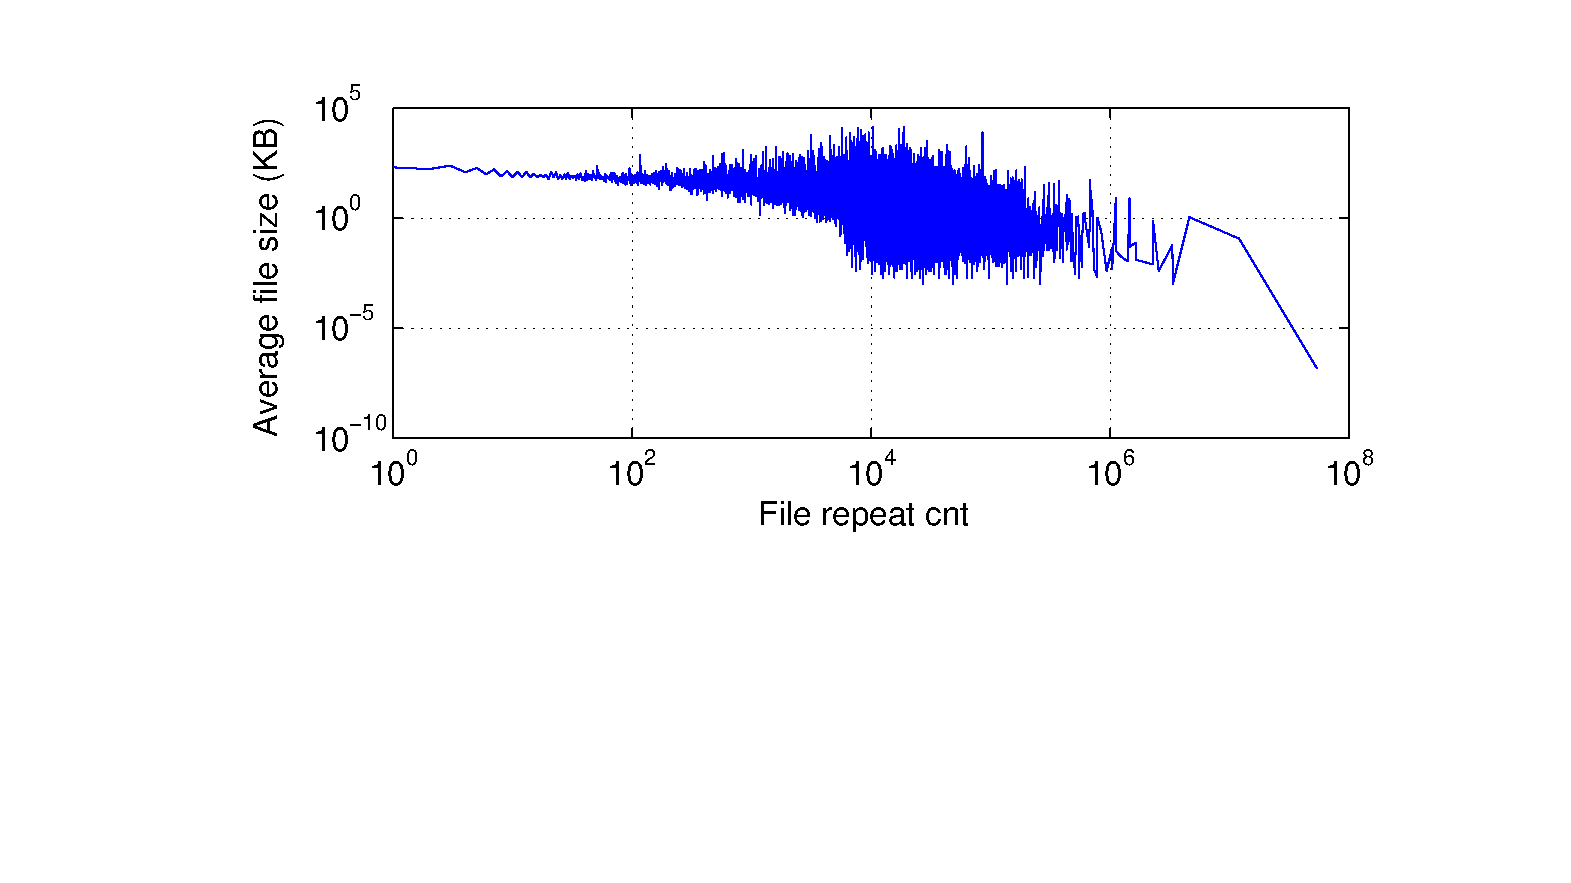
\includegraphics[width=0.5\textwidth]{graphs/avg_size_by_cnt.eps} %
%%\caption{Average file size with same repeat count.  %	} %
%%\label{fig_avg_size_by_cnt} %\end{figure} % %\paragraph{Redundant ratio by
%%file size for the files with the same content in terms of file count and
%%storage capacity} %Total size of redundant files with same content(TRS) %
%%%97\% of the TRSs are equal or less than 100MB.  % %\begin{figure} %
%%\centering %
%%\includegraphics[width=0.5\textwidth]{graphs/Total_size_of_redudant_files_with_same_content-KB.eps}
%%%	\caption{CDF of total file size with same file content (MB).  %	} %
%%\label{fig_total_redundant_same_digest} %\end{figure} % %\paragraph{Redundant
%%ratio by repeat count for the files with the same repeat count in terms of
%%file count and storage capacity} % %However, with the increase of file repeat
%%count, the sum of file size with same repeat count becomes smaller.  %
%%%\begin{figure} %	\centering %
%%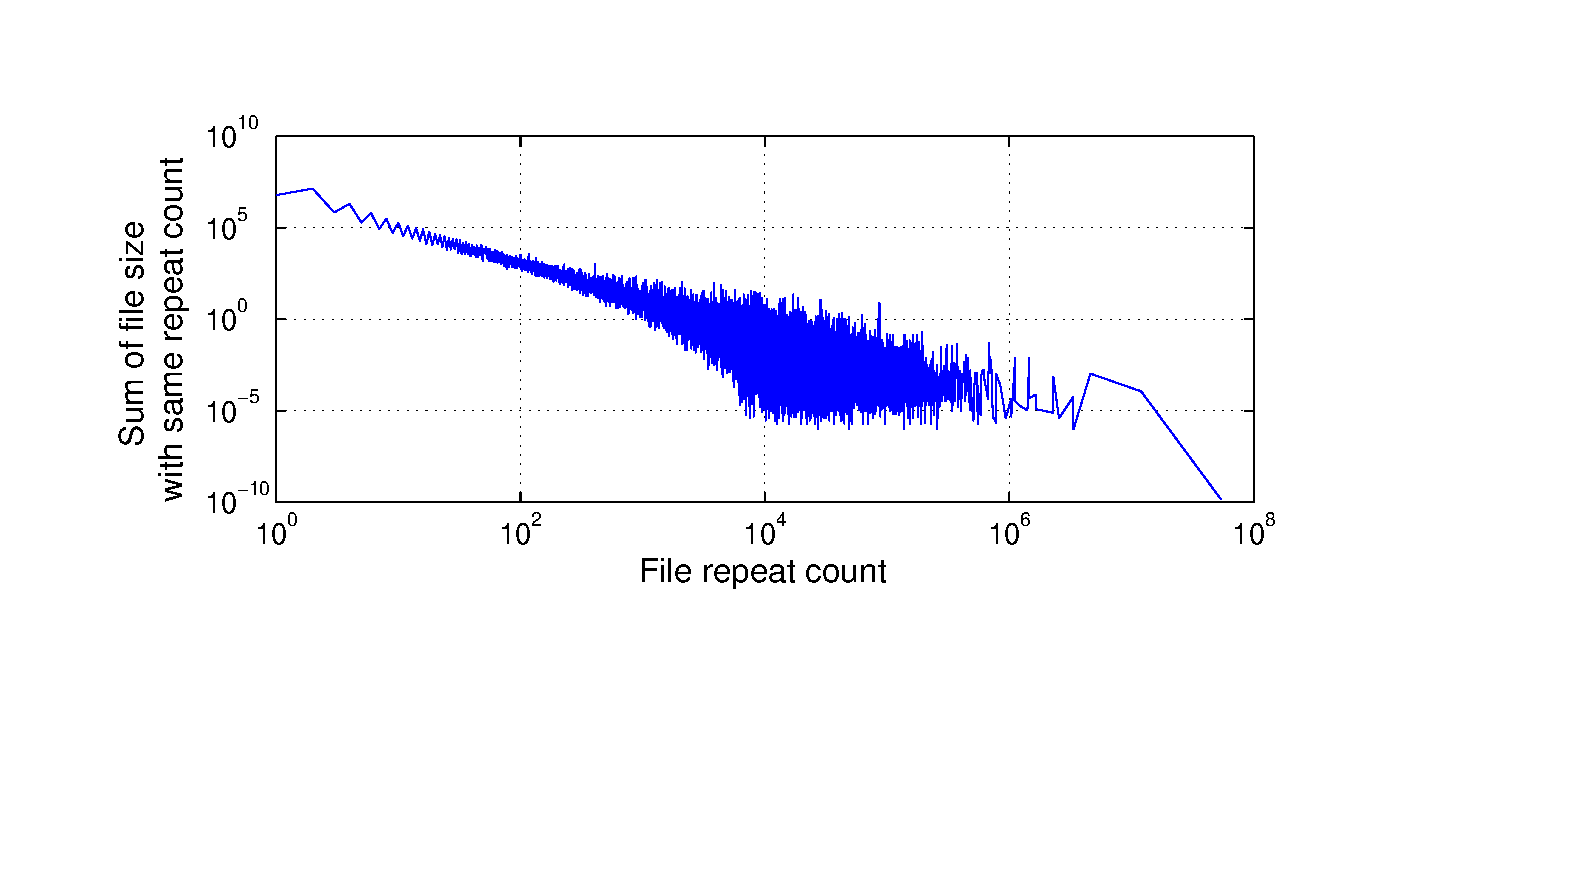
\includegraphics[width=0.5\textwidth]{graphs/sum_size_by_cnt.eps} %
%%\caption{Sum of file size with same repeat count.  %	} %
%%\label{fig_sum_by_cnt} %\end{figure}
%%
%%% %\paragraph{Cumulative distribution and probability distribution of file
%%repeat count} %\begin{table} %	\centering %	\scriptsize  %
%%%\begin{minipage}{.5\linewidth} %	\caption{Summary of image types}
%%\label{tbl:redundant_ratio} %	\begin{tabular}{|l|l|l|}%p{0.14\textwidth} %
%%\hline %		% after \\: \hline or \cline{col1-col2}
%%\cline{col3-col4} ...  %		% after \\: \hline or \cline{col1-col2}
%%\cline{col3-col4} ...  %		Image types & num. & avg. redundant
%%ratio  \\ %		\hline %		  &   &        \\ %
%%\hline %		  &   &         \\ %		\hline %
%%&   &       \\ %		   \hline %		other     &   &
%%\\ %		\hline %	\end{tabular} %\end{table}
%%
%%%\subsection{Redundant files with same filename and relative path} %
%%%\subsection{Common directories that contains redundant files} %
%%%\subsection{Redundant tar files} %\begin{table} %	\centering %
%%\scriptsize  %	%\begin{minipage}{.5\linewidth} %	\caption{Summary of
%%file \& dir. characterization} \label{tbl:sum_file_dir_char} %
%%\begin{tabular}{|l|l|l|l|l|}%p{0.14\textwidth} %		\hline %
%%% after \\: \hline or \cline{col1-col2} \cline{col3-col4} ...  %
%%% after \\: \hline or \cline{col1-col2} \cline{col3-col4} ...  %
%%Metrics & max & min & median & avg.\\ %		\hline %
%%File size &   &   &   &  \\ %		\hline %		File size
%%(repeat cnt. $>$ 1) &   &   &    &  \\ %		\hline %
%%File size (repeat cnt. $=$ 1) &   &   &    &  \\ %		\hline %
%%\hline %		Dir. size &  &  & & \\ %		\hline %
%%File cnt. per dir & &  &  & \\ %		\hline %
%%Redundant ratio & &  &  & \\ %		\hline %		Dir. depth  &
%%&  & & \\ %		\hline %	\end{tabular} %\end{table} 



%\section{Redundant file characterization}
\label{sec:redundant_files}

\subsection{File repeat count}

Almost 90\% of files have equal or less than 10 redundant copies. Most files have small repeat count.

\begin{figure}
	\centering
	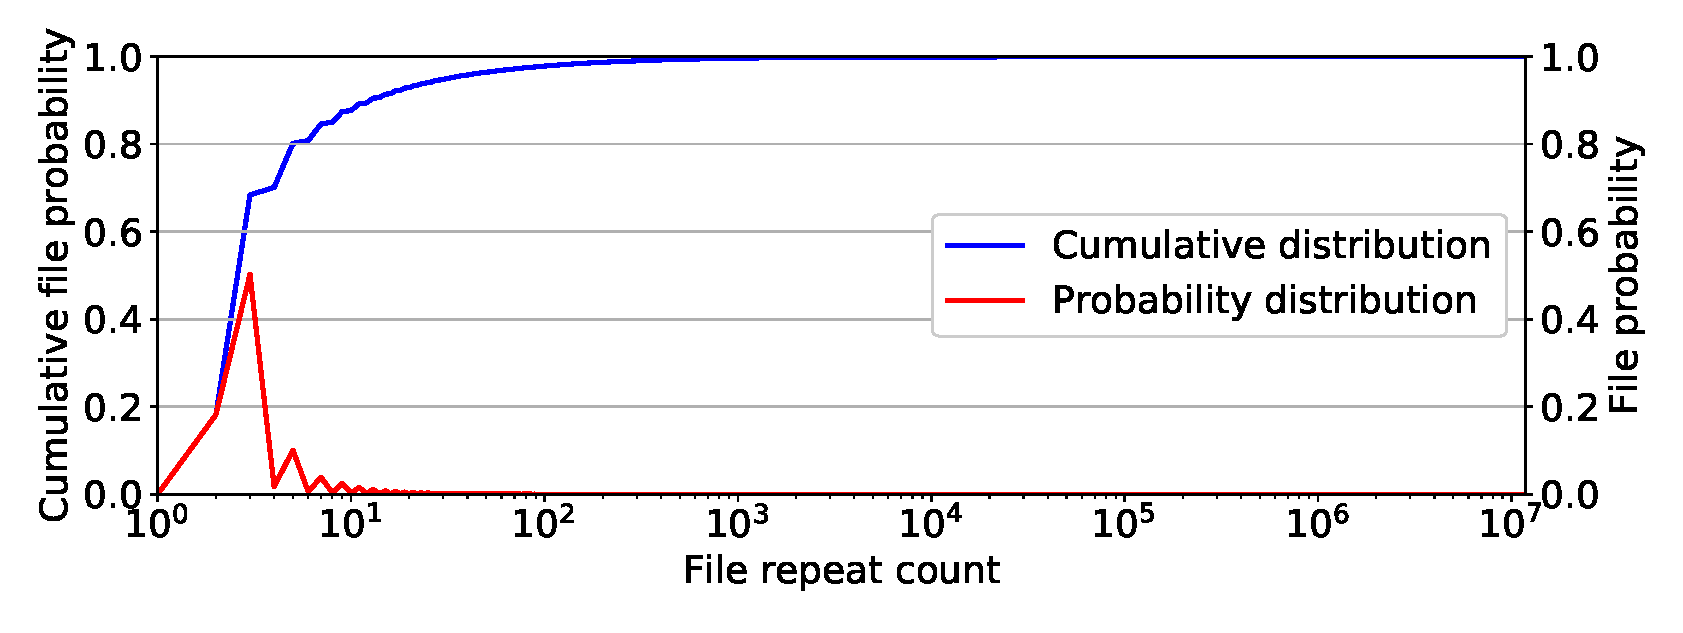
\includegraphics[width=0.5\textwidth]{graphs/File_repeat_count.eps}
	\caption{File repeat count distribution.
	}
	\label{fig:file_size}
\end{figure}

\subsection{File size}

91\% files'sizes are equal or less than 100KB. Most files are smaller files.

\begin{figure}
	\centering
	\includegraphics[width=0.5\textwidth]{graphs/File_size.eps}
	\caption{File size distribution.
	}
	\label{fig:file_size}
\end{figure}

%\begin{figure}
%	\centering
%	\subfigure[CDF of file size.]{\label{fig:dedup_cdf}
%		\includegraphics [width=0.5\textwidth]{graphs/file_repeat_cnt_cdf.eps}
%	}
%	\subfigure[PDF of file size.]{\label{fig:dedup_hist}
%		\includegraphics [width=0.5\textwidth]{graphs/file_repeat_cnt_pdf.eps}
%	}
%	\caption{File size distribution}
%	\label{fig:file_repeat_count}
%\end{figure}

\subsection{File type}

\paragraph{Top redundant file types}

Totally, we get around 690 types.

%\begin{table} 
%	\centering 
%	\scriptsize  
%	\caption{Top 20 redundant files' characterization (sorted by repeat cnt.)}
%	\label{tbl:top_dup_files_repeat_cnt} 
%	\begin{tabular}{|l|l|l|l|l|}%p{0.14\textwidth} 
%		\hline 
%		Filename & repeat cnt. & type & extension & size \\
%		\hline
%		&   &   &   &  \\
%		\hline
%		&   &   &   &   \\
%		\hline
%		&   &   &  &    \\
%		\hline
%		&  &  &  & \\
%		\hline
%		& &  &   & \\
%		\hline
%		& &  &   & \\
%		\hline
%		&  &  & & \\
%		\hline
%	\end{tabular} 
%\end{table}

%\begin{table} 
%	\centering 
%	\scriptsize  
%	\caption{Top 20 redundant files' characterization (sorted by capacity)} 
%	\label{tbl:top_dup_files_cap} 
%	\begin{tabular}{|l|l|l|l|l|}%p{0.14\textwidth} 
%		\hline 
%		Filename & repeat cnt. & type & extension & size \\
%		\hline
%		&   &   &   &  \\
%		\hline
%		&   &   &   &   \\
%		\hline
%		&   &   &  &    \\
%		\hline
%		&  &  &  & \\
%		\hline
%		& &  &   & \\
%		\hline
%		& &  &   & \\
%		\hline
%		&  &  & & \\
%		\hline
%	\end{tabular} 
%\end{table}


%\begin{table} 
%	\centering 
%	\scriptsize  
%	\caption{Top redundant file types} 
%	\label{tbl:top_dup_types} 
%	\begin{tabular}{|l|l|l|l|l|l|}%p{0.14\textwidth} 
%		\hline 
%		Type & extension & Num. & size & red. ratio (cnt.)  & red. ratio (cap.)\\
%		\hline
%		&   &   &  & &   \\
%		\hline
%		&   &   &  & &    \\
%		\hline
%		&   &   &   & &   \\
%		\hline
%		&  &  &  & & \\
%		\hline
%		& &  &  & & \\
%		\hline
%		& &  & & &  \\
%		\hline
%		&  &  & & &  \\
%		\hline
%	\end{tabular} 
%\end{table} 

%\subsection{Redundant ratio for directories}
%
%\begin{table} 
%	\centering 
%	\scriptsize  
%	%\begin{minipage}{.5\linewidth}
%	\caption{Inter-dir redundant ratio for dirs in terms of file count and capacity} \label{tbl:intra_dup_ratio_dirs} 
%	\begin{tabular}{|l|l|l|}%p{0.14\textwidth} 
%		\hline 
%		% after \\: \hline or \cline{col1-col2} \cline{col3-col4} ... 
%		% after \\: \hline or \cline{col1-col2} \cline{col3-col4} ... 
%		& File count & Capacity \\
%		\hline
%		Avg. & 98.75\% & 97.33\%\\
%		\hline
%		Median & - & - \\
%		\hline
%		Max. & 1 & 1\\
%		\hline
%		Min.  & 0.87\%  & $<$ 0.00\%\\
%		\hline
%		Stdev.  &  4.70\% & 10.49\\
%		\hline
%		Layer dataset after share.-dedup (Uncompressed) & -  & -\\
%		\hline 
%		Total layer dataset (Uncompressed) &  -	& -\\
%		\hline
%	\end{tabular} 
%\end{table}
%
%\begin{table} 
%	\centering 
%	\scriptsize  
%	%\begin{minipage}{.5\linewidth}
%	\caption{Intra-dir redundant ratio for dirs in terms of file count and capacity} \label{tbl:inter_dup_ratio_dirs} 
%	\begin{tabular}{|l|l|l|}%p{0.14\textwidth} 
%		\hline 
%		% after \\: \hline or \cline{col1-col2} \cline{col3-col4} ... 
%		% after \\: \hline or \cline{col1-col2} \cline{col3-col4} ... 
%		& File count & Capacity \\
%		\hline
%		Avg. & 98.75\% & 97.33\%\\
%		\hline
%		Median & - & - \\
%		\hline
%		Max. & 1 & 1\\
%		\hline
%		Min.  & 0.87\%  & $<$ 0.00\%\\
%		\hline
%		Stdev.  &  4.70\% & 10.49\\
%		\hline
%		Layer dataset after share.-dedup (Uncompressed) & -  & -\\
%		\hline 
%		Total layer dataset (Uncompressed) &  -	& -\\
%		\hline
%	\end{tabular} 
%\end{table}

%\subsection{Redundant directory characterization}
%
%\begin{table} 
%	\centering 
%	\scriptsize  
%	%\begin{minipage}{.5\linewidth}
%	\caption{Top redundant dirs'characterization} 
%	\label{tbl:top_dup_dirs} 
%	\begin{tabular}{|l|l|l|l|}%p{0.14\textwidth} 
%		\hline 
%		% after \\: \hline or \cline{col1-col2} \cline{col3-col4} ... 
%		% after \\: \hline or \cline{col1-col2} \cline{col3-col4} ... 
%		Name & Num. & Redundant ratio & Avg. size \\
%		\hline
%		home &   &   &     \\
%		\hline
%		&   &   &      \\
%		\hline
%		&   &   &      \\
%		\hline
%		&  &  &  \\
%		\hline
%		& &  &   \\
%		\hline
%		& &  &   \\
%		\hline
%		&  &  & \\
%		\hline
%	\end{tabular} 
%\end{table} 

%=======================================
%|             OLD VERSION              |
%=======================================

%\begin{figure}
%	\centering
%	\includegraphics[width=0.5\textwidth]{graphs/}
%	\caption{CDF of file repeat count.
%	}
%	\label{fig:file_repeat_count}
%\end{figure}

%\paragraph{Cumulative distribution and probability distribution of file size in terms of unique file size, redundant file size, overall file size}


%\paragraph{Average file size by repeat count}
%
%There is no relation between file repeat count and average file size.
%
%\begin{figure}
%	\centering
%	\includegraphics[width=0.5\textwidth]{graphs/avg_size_by_cnt.eps}
%	\caption{Average file size with same repeat count.
%	}
%	\label{fig_avg_size_by_cnt}
%\end{figure}
%
%\paragraph{Redundant ratio by file size for the files with the same content in terms of file count and storage capacity}
%Total size of redundant files with same content(TRS)
%
%97\% of the TRSs are equal or less than 100MB.
%
%\begin{figure}
%	\centering
%	\includegraphics[width=0.5\textwidth]{graphs/Total_size_of_redudant_files_with_same_content-KB.eps}
%	\caption{CDF of total file size with same file content (MB).
%	}
%	\label{fig_total_redundant_same_digest}
%\end{figure}
%
%\paragraph{Redundant ratio by repeat count for the files with the same repeat count in terms of file count and storage capacity}
%
%However, with the increase of file repeat count, the sum of file size with same repeat count becomes smaller.
%
%\begin{figure}
%	\centering
%	\includegraphics[width=0.5\textwidth]{graphs/sum_size_by_cnt.eps}
%	\caption{Sum of file size with same repeat count.
%	}
%	\label{fig_sum_by_cnt}
%\end{figure}

%
%\paragraph{Cumulative distribution and probability distribution of file repeat count}
%\begin{table} 
%	\centering 
%	\scriptsize  
%	%\begin{minipage}{.5\linewidth}
%	\caption{Summary of image types} \label{tbl:redundant_ratio} 
%	\begin{tabular}{|l|l|l|}%p{0.14\textwidth} 
%		\hline 
%		% after \\: \hline or \cline{col1-col2} \cline{col3-col4} ... 
%		% after \\: \hline or \cline{col1-col2} \cline{col3-col4} ... 
%		Image types & num. & avg. redundant ratio  \\
%		\hline
%		  &   &        \\
%		\hline
%		  &   &         \\
%		\hline
%		   &   &       \\
%		   \hline
%		other     &   &       \\
%		\hline
%	\end{tabular} 
%\end{table}

%\subsection{Redundant files with same filename and relative path}
%
%\subsection{Common directories that contains redundant files}
%
%\subsection{Redundant tar files}
%\begin{table} 
%	\centering 
%	\scriptsize  
%	%\begin{minipage}{.5\linewidth}
%	\caption{Summary of file \& dir. characterization} \label{tbl:sum_file_dir_char} 
%	\begin{tabular}{|l|l|l|l|l|}%p{0.14\textwidth} 
%		\hline 
%		% after \\: \hline or \cline{col1-col2} \cline{col3-col4} ... 
%		% after \\: \hline or \cline{col1-col2} \cline{col3-col4} ... 
%		Metrics & max & min & median & avg.\\
%		\hline
%		File size &   &   &   &  \\
%		\hline
%		File size (repeat cnt. $>$ 1) &   &   &    &  \\
%		\hline
%		File size (repeat cnt. $=$ 1) &   &   &    &  \\
%		\hline
%		\hline
%		Dir. size &  &  & & \\
%		\hline
%		File cnt. per dir & &  &  & \\
%		\hline
%		Redundant ratio & &  &  & \\
%		\hline
%		Dir. depth  &  &  & & \\
%		\hline
%	\end{tabular} 
%\end{table} 
%%\section{Image characterization}
%\label{sec:redundant_images}
%
%\subsection{Layer count}
%
%\subsection{Image size}
%
%\subsection{Compression ratio}
%
%\subsection{Directory count}
%
%
%\subsection{File count}



\section{Slimmer design}
\label{sec:slimmer}

%Our analysis in Section~\ref{sec:redundant_files} suggests that adding the
%support of file-level deduplication to Docker registry can significantly reduce
%its storage capacity requirements, especially in large-scale deployments.
%
In this section, we first describe a high-level design of \emph{\sysname}---
a Docker registry that supports file-level deduplication.
We then proceed with a simulation-based evaluation of the expected performance
implications.

Integrated Caching and Deduplication

Cache-assisted Inline deduplication system



\subsection{Design}
\label{sec:design}

We designed \sysname\ so that the interface between the Docker clients and the
registry remains unchanged.
%
As such, no modifications are needed in the Docker clients.
%
Below we describe the actions that \sysname\ takes during the layer pushes and
pulls at the registry side.
%
For the sake of this paper, we explain only the main steps omitting smaller
details.

\paragraph{Push}
%
\sysname\ does not unpack the layer immedieately after receiving it from a
client.
%
Instead, \sysname\ saves the layer's compressed tarball in a persistent
\emph{staging area}.
%
A separate \emph{off-line} deduplication process iterates over the layers in
the staging area and performs the following actions for every layer:
%
\textbf{1)}~uncompresses and unpacks the layer's tarball into individual files;
%
\textbf{2)}~computes a \emph{fingerprint} for every file in the layer;
%
\textbf{3)}~checks all file fingerprints against the \emph{file index} to
identify if identical files are already stored in \sysname;
%
\textbf{4)}~stores non-deduplicated files in \sysname's storage system;
%
\textbf{5)}~creates and stores a \emph{layer recipe} that includes the path,
metatada, and fingerprint of every file in the layer;
%
\textbf{6)}~removes the layer's tarball from the staging area.

We believe that off-line deduplication is appropriate because it keeps push
latencies percieved by the Docker clients low.
%
Background deduplication process can be scheduled during the periods of low
load on the registry.
%
Layer recipies are identified by layer's digests (Section~\ref{sec:background})
and files are identified by their fingeprints.
%
These identifiers are used to store and retrieve corresponding objects in the
underlying storage.
%
For example, if a file system is used as a backend storage, \sysname\ creates a
single file for  every layer recipe (named by the digest) and a single file for
every in-layer file (named by the fingerprint).


\paragraph{Pull}
%
Pulling the layer cannot be postponed to the off-line process becasue the
Docker client is actively waiting for the layer. 
%
\sysname\ performs the following actions \emph{inline} during the pull request:
%
\textbf{1)}~if a layer is still in the staging area, \sysname\ services it
directly form there;
%
\textbf{2)}~otherwise, \sysname\ finds the layer recipe by the layer digest
(provided by the client);
%
\textbf{3)}~prepares a directory structure for the layer based on the layer
recipe;
%
\textbf{4)}~packs and compresses the layer's  directory tree into a temporary
tarball;
%
\textbf{5)}~sends the layer tarball back to the client;
%
\textbf{5)}~disards the layer tarball.



\subsection{Performance Evaluation}

While \sysname\ can effectively eliminate redundant files in the
Docker registry, it introduces overheads which can reduce the
registry's performance.
%
%The overheads can be classified in two categories: 1)~\emph{background
%overhead} caused by the computation and I/O that is performed during layer
%deduplication; and 2)~\emph{foreground overhead} from extra processing on the
%critical path of a pull request.

\begin{figure}
	\centering
	\includegraphics[width=0.48\textwidth]{graphs/res-time.pdf}
	\caption{Off-line file-level deduplication run time.}
	\label{fig:dedup-res}
\end{figure}


\paragraph{Simulation}
%
To analyze the impact of file-level deduplication on performance,
we conducted a preliminary simulation of \sysname.
%
%Based on the simulation results, we estimated the overhead of \sysname\ on
%\texttt{push} and \texttt{pull} layer request latencies.
%
%We then provide different suggestions on how the Docker registry can mitigate
%the deduplication overhead.
%
%%%%%%%%%%%%%%%%%%%%%%%%%%%%%%%%%%%%%%%%%%%%%%%%%%%%%%%%%%%%%%%%%%%%%%%%%%%%
%
%
Our simulation
approximates several \sysname's steps described in Section~\ref{sec:design}.
%
First, a layer from our dataset is copied to a RAM disk. 
%
%
%Note that there is no foreground pull or push requests since the simulation is \emph{off-line}.
%
The layer is then decompressed, unpacked, and the fingerprints of all files
are computed using the MD5 hash function~\cite{MD5}.
%
The simulation searches the fingerprint index for duplicates,
and, if the file has not been stored previously, it records the
file's fingerprint in the index.
%
%To map a layer to its containing files, we create the layer recipe and add it
%to a \emph{layer-to-file table}.
%
%The simulator then creates a file recipe.
%
%For each file in a layer, a layer digest
%to its containing file content digest mapping record is also created 
%
%The \emph{layer-to-file table} also
%records the file path within each layer associated with each file.
%
Note that at this point our simulation does not include
the latency of storing unique files.
%
To simulate layer's reconstruction during the \texttt{pull},
we archive and compress corresponding files.
%
%Only unique files are maintained in RAM
%disk while the redundant copies are removed.
%

We implemented the simulation in 600 lines of Python code
and setup a one-node Docker registry on a machine with 32~cores and 64GB of RAM.
%
To speed up the experiments and fit the required data in the RAM
we used 50\% of all layers and excluded the ones larger than 50MB.
%
We processed 60 layers in parallel using 60 threads.
%
The overall runtime of the simulation was roughly 3.5 days.
%
%The overall runtime is about 3.5 days.

Figure~\ref{fig:dedup-res} shows the CDF for each sub-operation of
\sysname.
%
Unpacking, Decompression, Digest Calculation, and Searching 
are part of
the deduplication process and together make up the Dedup time.
%
\VT{@Nannan, in Figure ~\ref{fig:dedup-res} can you reorder the lines in the
legend so that the Searching goes after Digest calculation?}
%
Searching, Archiving, and Compression
simulate the additional processing for a \texttt{pull}
request and form the Pulling time.
%

%\LR{What was the overall runtime for processing 0.9 million layers?}\NZ{addressed}
%
%\alicomment{How are we saving the location
%of each file in the layer? It is not clear from the following sentences.}
%\NZ{addressed}
%
%To improve searching performance, the
%mapping table is stored in Hive database~\cite{xxx}. 
%
%\lrcomment{Why are we using Hive for this? It seems overkill to me, especially
%for such small data. Even at scale, a KeyValue store would probably provide
%better performance than clunky MapReduce-based DB.}
%

\paragraph{Push}

\sysname\ does not directly impact the latency of \texttt{push} requests because
deduplication is performed asynchronously, \ie the registry reliably stores a
copy of the layer as-is and then sends a response to the client.
%
The appropriate performance metric for push is the time it takes to deduplicate
a single layer.
%
%Next, we look at the effects on \texttt{push} and \texttt{pull} latencies in
%more detail.
%
%However, if there are intensive push requests while the registry is performing
%deduplication, \sysname\ can still impact push latencies because it incurs
%CPU, memory, and I/O overhead. %(similar to pull requests).
%
Looking at the breakdown of the deduplication time in
Figure~\ref{fig:dedup-res}, we make several observations.
%
First, the searching time is the smallest among all operations with 90\% of the
searches completing in less than 4ms and the median of \VT{XXX}ms.
%
%The mapping table maintains 0.98 million layer-to-file digest mapping records. 
%
%\LR{Remove the following sentence? 1.7 million records is actually quite small
%so even a single-node DB with one index is enough.}\NZ{addressed} Consider
%that more than 1.7 million layers are stored in Docker hub and the number is
%still increasing, it's better to choose a fast distributed database to provide
%high searching performance and scalability.
%
Second, the calculation of digests spans a wide range from 5$\mu$s to almost
125s.
%
%This is because the time mainly depends on the layer size, \ie the fewer and
%smaller files a layer contains, the faster it is to compute all digests for
%the layer.
%
%Typically, smaller layers contain a smaller number of smaller files, which
%takes much less time to calculate their digests.
%
%While if the layer is bigger, the digest calculation overhead will be higher. 
%
90\% of digest calculation times are less than 27s while 50\% are
less than \VT{XXX}s.
%
The diversity in the timing is caused by a high variety of layer sizes both in
terms of storage space and file counts.
%
%Thus, we suggest that multiple-threading is needed to calculate the files'
%digests simultaneously; 
%
%Fast CPUs as well as more powerful computing nodes are required to speed up
%digest calculation.
%
Third, the run time for decompression and unpacking follows identical
distribution for approximately 60\% of the layers and is less than 150ms.
%
%Around 60\% of decompression and unpacking time are less than 0.15\,s. 
%
However, after that, the times diverge and compression times increase faster
compared to unpacking times.
%
\VT{do we have some theory why?}
%
90\% of decompressions take less than 950ms while 90\% of packing time is less
than 350ms.

%Overall, we see that file digest calculation contributes a lot to the
%overall deduplication latency especially when the layer size is big.  Moreover,
%we see that the deduplication latency increases as the layer size grows.
%
Overall, we see that 90\% of file-level deduplication time is less than \VT{XXX}s
per layer, while the average processing time for a single layer is \VT{XXX}.
%
This means that our single-node deployment can process about 3 layers/s on average.
%
In future we will work on further improving \sysname's deduplication throughput.
%
%In a large-scale registry deployment, this throughput can be improved
%as more node are available to perform deduplication.
%

\paragraph{Pull layer latency} 

For a \emph{pull layer} requests, \sysname\ will first fetch 
all its containing files by consulting the \emph{layer-to-file table}, 
restore the layer archive file and then send the compressed archive back
to the clients.

Figure~\ref{fig:dedup-res} shows the latency distributions for the compression
and archiving steps.
%
%Note that the \emph{pull layer} latency is the sum of archiving time,
%compression time, and searching time and does not include network transfer
%time.
%
%\LR{Always add a protected space or a \textbackslash, between a number and its unit.}
%\NZ{addressed}
%
We can see that around 55\% of the layers have a similar compression and archiving
time ranging from from 0.04\,s to 0.15\,s and both operations contribute equally
to pulling latency.
%60\% of compression and archiving time are less than 0.15 s.
%
%While compression has the highest run time 80\% of compression time is less than 2.82~s. 
%
\LR{Again, better to show the 90th percentile.}
\NZ{90\% of the compression time is less than 8\,s.}
After that, the times diverge and compression times increase faster with an
80\textsuperscript{ts} percentile of 2.82\,s.
%
Hence, compression time makes up the major portion of the pull latency and becomes a
bottleneck.
%
This is because compression times increase for larger layers and follow the distribution
of layer sizes (see Figure~\ref{fig:layer-size-cdf}).
%\LR{put reason here}
%\NZ{I think the layer size is the major reason}.
%
%We see that archiving time and compression contributes equally to pulling
%latency when their run time are lower than 0.15 s while compression time almost
%equals to pulling latency when the compression time is greater than 0.15 s. 

\LR{Should we move that to 4.3?}
%
\NZ{Can we use it as conclusion}
To reduce latency, we suggest that fast compression methods should be applied to reduce
compression times. As deduplication provides significant storage savings, faster compression
methods with a lower compression ratio are hence feasible.

%\alicomment{Separately mention pull layer requests}
%

%\paragraph{File-level deduplication run time}


\section{Discussion}

We propose additional optimizations that can help to speed up \sysname:

\begin{compactenumerate}
%
\item
%
As the majority of the pull time is caused by compression, we propose to cache
hot layers as precompressed tar files in the staging area.
%
%We observe that only a small proportion of images and layers are frequently
%requested and majority of images and layers are \textit{cold}.
%
%Figure~\ref{fig:pull-cnt} shows the total number of pulls from the time an
%image/layer has been stored in Docker Hub until May 30, 2017.
%
According to our statistics, only 10\% of all images were pulled
from Docker Hub more than 360 times from the time the image was first pushed to Docker Hub
until May 30, 2017. Moreover, we found that 90\% of pulls
went to only 0.25\% of images based on image pull counts.
%
This suggests the existence of both cold and hot images and layers.
%
%\VT{Nannan, can we instead compute that 90\% of pulls
%wen to 0.25\% of images?}
%
%
%translates to only 10\% of layers being pulled more than 660 times (at most).
%
%Note that we calculate the layer pull count shown in Figure~\ref{fig:pull-cnt}
%by aggregating the pull count of all images, which refer to this layer.
%
%Note that the image pull counts are crawled from Docker Hub website.
%
%Actual layer pull counts should be less because pulling an image does not
%necessarily pull all its containing layers if some layer have been previously
%downloaded and are already available locally.
%

\item
%
As deduplication provides significant storage savings, \sysname\ can use faster
but less effective local compression methods than gzip~\cite{lz4}.
%
%\VT{cite a few}

\item
%
%Deduplicating when workload is light As shown above, file-level deduplication
%comes with some performance overhead.
%
The registries often experience fluctuation in load with peaks and
troughs~\cite{dockerworkload}.
%
Thus, file-level deduplication can be triggered
when the load is low to prevent interference with 
client \texttt{pull} and \texttt{push} requests.
%
%To further improve the performance of \sysname\, we also suggest to use main
%memory for temporarily storing and processing \textit{small} layers.
%
%According to our findings (see~\S\ref{sec:dedup_ratio}), the majority of
%layers~(87.3\%) are smaller than 50\,MB and hence can be stored and processed
%in RAM to speed up deduplication. 
%
\end{compactenumerate}

%\begin{figure}
	\centering
	\includegraphics[width=0.4\textwidth]{graphs/pull-cnt.pdf}
	\caption{CDF of layer \& image pull count.
	}
	\label{fig:pull-cnt}
\end{figure}

%=======================================
%|             OLD VERSION              |
%=======================================

%\paragraph{Latency distribution for each operation}
%\subsubsection{When to start file-level dedup?} 

%\paragraph{Latency distribution for each operation}

%\paragraph{Small compression ratio and small layer size}
%
%\begin{figure}[!t]
	\centering
	\subfigure[CDF of compression ratio]{\label{fig_cdf_compression_ratio}
		\includegraphics[width=0.23\textwidth]{graphs/cdf_compression_ratio.pdf}
	}
	\subfigure[Histogram of comp. ratios]{\label{fig_his_compression_ratio}
		\includegraphics[width=0.223\textwidth]{graphs/his_compression_ratio.pdf}
	}
	\caption{Layer compression ratio distribution
	\vcomment{Different colors are used in figure (a) and (b) FLS/CLS}
	}
	\label{fig-compression-ratio}
\end{figure}

%
%\begin{figure}[!t]
	\centering
	\subfigure[CDF of layer sizes]{\label{fig_layer_size_cdf}
		\includegraphics[width=0.234\textwidth]{graphs/layer_size_mb.pdf}
	}
	\subfigure[Histogram of layer sizes]{\label{fig_hist_layer_size}
		\includegraphics[width=0.213\textwidth]{graphs/hist_layer_size.pdf}
	}
	\caption{Layer size distribution
%	\vcomment{Let's use CLS, ALS, and FLS abreviations\nancomment{addressed}}.
%	\vcomment{CLS size should go first}.
%	\vcomment{We need to use different types of lines (solid, dotted, etc.)
%		or markers (round, triangular)}.
%	\vcomment{In figure B it is not clear to which bar group corresponds
%		  to which layer size. I suggest to try to rotate the graph
%		  by 90 grads to fit all layer size labels.\nancomment{aligned label with bar}}
	}
	\label{fig-layer-size}
\end{figure}

%
%We found that most layers'compression ratio is really lower (?) while most of layers have a smaller size. 
%So how about we use archiving instead of compression if the network speed is higher (?GB/s)?

%\paragraph{Network transfer speed is high!}

%\subsubsection{File-level content addressable storage for cold layers}

%\begin{figure}
%	\centering
%	\includegraphics [width=0.45\textwidth]{plots/exp-total-stev-erase.eps}
%	\subfigure[]{\label{fig:per_layer_ratio_fcnt_cdf}
%		\includegraphics [width=0.23\textwidth]{graphs/}
%	}
%	\subfigure[Similar layer dedup]{\label{fig:per_layer_ratio_fcnt_pdf}
%		\includegraphics [width=0.22\textwidth]{graphs/graph_reconstruct_layers.pdf}
%	}
%	\caption{File-level content addressable storage model}
%	\label{fig:eval-stdev-erasure-cnt}
%\end{figure}

%\subsection{Hints for performance improvement and storage saving}

%\begin{table} 
%	\centering 
%	\scriptsize  
%	%\begin{minipage}{.5\linewidth}
%	\caption{Latency breakdown} \label{tbl:latency_breakdown} 
%	\begin{tabular}{|l|l|l|l|l|}%p{0.14\textwidth} 
%		\hline 
%		% after \\: \hline or \cline{col1-col2} \cline{col3-col4} ... 
%		% after \\: \hline or \cline{col1-col2} \cline{col3-col4} ... 
%		Operations/latency (S) & max & min & median & avg.\\
%		\hline
%		 gunzip decompression (RAM) & 257.16  & 0.04  & 0.15  & 0.39 \\
% 		\hline
% 		tar extraction (RAM) & 43.41  & 0.04  &  0.14  & 0.18 \\
%		\hline
%		Digest calculation (RAM) & 3455.01  & $<$0.00  & 0.05 & 10.65 \\
%		\hline
%		tar archiving (RAM)  & 53.44 & 0.04 & 0.14 & 0.19\\
%		\hline
%		gzip compression (RAM) & 496.04 & 0.04 & 0.15 & 2.10 \\
%%		\hline
%%		Total time (RAM) (with compression) & & & & \\
%%		\hline
%%		Total time (RAM) (without compression) & & & & \\
%		\hline
% 		\hline
% 		gunzip decompression (SSD) &   &   &    &  \\
% 		\hline
% 		tar extraction (SSD) &   &   &    &  \\
%		\hline
%		Digest calculation (SSD) &  &  & & \\
%		\hline
%		tar archiving (SSD) &  &  & & \\
%		\hline
%		gzip compression (SSD) & &  &  & \\
%%		\hline		 
%%		Total time (SSD) (with compression) & & & & \\
%%		\hline
%%		Total time (SSD) (without compression) & & & & \\
%		\hline
%		\hline
%		Network transfer & 20587.94 & $<$ 0.00 & $<$ 0.00 & 1.20 \\
%		\hline 	
%	\end{tabular} 
%\end{table}


%\begin{table} 
%	\centering 
%	\scriptsize  
%	%\begin{minipage}{.5\linewidth}
%	\caption{Summary of layer \& image characterization} \label{tbl:redundant_ratio} 
%	\begin{tabular}{|l|l|l|l|l|}%p{0.14\textwidth} 
%		\hline 
%		% after \\: \hline or \cline{col1-col2} \cline{col3-col4} ... 
%		% after \\: \hline or \cline{col1-col2} \cline{col3-col4} ... 
%		Metrics & max & min & median & avg.\\
%		\hline
%		Compressed layer size &   &   &   &  \\
%		\hline
%		Uncompressed layer size &   &   &    &  \\
%		\hline
%		Archival size &  &  & & \\
%		\hline
%		Compression ratio &   &   &    &  \\
%		\hline
%		Layer pull cnt. &  &  & & \\
%		\hline
%		File cnt. per layer &  &  & & \\
%		\hline
%		Dir. cnt. per layer &  &  & & \\
%		\hline
%		Layer depth &  &  & & \\
%		\hline
%		\hline
%		Compressed image size &  &  & & \\
%		\hline
%		Uncompressed image size & &  &  & \\
%		\hline
%		Archival image size & &  &  & \\
%		\hline
%		Compression ratio &   &   &    &  \\
%		\hline
%		Image pull cnt.  &  &  & & \\
%		\hline
%		Layer cnt. per image  &  &  & & \\
%		\hline
%		Shared layer cnt. per image  &  &  & & \\
%		\hline
%		File cnt. per layer &  &  & & \\
%		\hline
%		Dir. cnt. per layer &  &  & & \\
%		\hline	
%	\end{tabular} 
%\end{table} 

%\subsection{Constructing shared layers for redundant directories/files}
%
%\paragraph{Smaller number of layers are shared among different images}
%\begin{figure}[!t]
	\centering
	\subfigure[CDF of layer by layer count]{\label{fig_repeate_layer}
		\includegraphics[width=0.23\textwidth]{graphs/repeate_layer.pdf}
	}
	\subfigure[Histogram of images by layer count in images]{\label{fig_hist_repeate_layer}
		\includegraphics[width=0.223\textwidth]{graphs/hist_repeate_layer.pdf}
	}
	\caption{Compression rate distribution}
	\label{fig-repeat-layer-cnt}
\end{figure}
%
%\paragraph{Smaller pull latency than recompression model} the registry can prepare the reconstructed layers before users issue a pull request. But this model requires users to rebuild two layers.

%\subsubsection{Summary of Suggestions/trade-offs between dedup ratio and recompression overhead}
%
%\paragraph{1. using archiving instead of compression}
%\paragraph{2. using file-level dedup for cold images/layers}
%\paragraph{3. using file-level dedup economically}
%When to trigger file-level dedup?
%\paragraph{4. constructing shared layers for redundant dirs/files, for example,}
%%\subsection{Layer reconstruction model}
%%\subsubsection{Reconstruction overhead}
%%\subsubsection{Trade-offs between dedup ratio and reconstruction overhead}
%%\paragraph{Dedup ratio VS. Rebuild overhead}
%%\subsection{Evaluation results}


%\section{Characterization}
\label{sec:char}

In this section we perform storage-oriented characterization of the Docker Hub
dataset and draw our insights.
%
After presenting registry growth trends, we characterize layers
(\S~\ref{sec:layers}) and then proceed to images (\S~\ref{sec:images}).
%
\paragraph{Docker Hub growth.} Figure~\ref{fig_image_growth} shows the total
number of repositories in Docker Hub from May 30 to September 20, 2017.
%
%As discussed in~\cite{XXX}, Crawler searched for `/' by using Docker hub
%search engine, crawled the web page, and obtained the total number of
%non-official public repositories in Docker hub each day. By summing both
%official repository count and non-official repository count, we got the total
%number of repositories in Docker hub each day.
%
During this 110-day period the total number of repositories increased from
633,915 to 687,292, resulting to 1,241 repositories created per day on average.
%
The graph is missing the points for the July 11 to July 26 because Docker Hub
stopped indexing ``/'' symbol in the repository names (which we originally used
to search for repositories).
%
We noticed this issues on July 26 and started to use ``*'' symbol for search
instead.


\begin{figure}
  \centering
  \includegraphics[width=0.5\textwidth]{graphs/image_growth.pdf}
  \caption{Total number of public repositories in Docker Hub
	   from May 30 to September 20, 2017. Y axis starts
	   at 630,000 repositories.
	   \vcomment{X axis label should be ``Date''.}
	   \vcomment{Y axis label x100,000 ``is badly aligned''.}
	   \vcomment{Y axis label x100,000 ``is badly aligned''.}
	  }
  \label{fig_image_growth}
\end{figure}

\subsection{Layers}
\label{sec:layers}

\paragraph{Layer size}

\begin{figure}[!t]
	\subfigure[CDF of layer size]{\label{fig_layer_size}
		\includegraphics[width=0.4\textwidth]{graphs/layer-size-cdf.pdf}
		}
		\centering
		\subfigure[CDF of image size]{\label{fig_image_size}
			\includegraphics[width=0.4\textwidth]{graphs/image-size-cdf.pdf}%
			}
			
			\caption{Image/layer size distribution}
			\label{fig:image-layer-size}
			\end{figure}

\paragraph{Layer directory depth}
%\nancomment{fs metadata overhead}

\begin{figure}[!t]
	\centering
	\subfigure[CDF of layer depth]{\label{fig_reference_cnt_cdf}
		\includegraphics[width=0.21\textwidth]{graphs/layer-depth-cdf.pdf}%
	}
	\subfigure[Histogram of layer depth]{\label{fig_reference_cnt_pdf}
		\includegraphics[width=0.21\textwidth]{graphs/layer-depth-pdf.pdf}
	}
	\caption{Layer depth distribution}
	\label{fig:reference-cnt}
\end{figure}

\paragraph{Directory count and File count}
%\nancomment{how union fs handle so large dirs}
\begin{figure}
	\centering
	\includegraphics[width=0.4\textwidth]{graphs/dir-cnt-cdf.pdf}
	\caption{CDF of directory count per image/layer.
	}
	\label{fig:reference-cnt}
\end{figure}

\begin{figure}[!t]
	\centering
	\subfigure[Histogram of directory count per image]{\label{fig_reference_cnt_cdf}
		\includegraphics[width=0.2\textwidth]{graphs/image-dir-cnt-pdf.pdf}%
	}
	\subfigure[Histogram of directory count per layer]{\label{fig_reference_cnt_pdf}
		\includegraphics[width=0.22\textwidth]{graphs/layer-dir-cnt.pdf}
	}
	\caption{Histogram of directory count distribution}
	\label{fig:reference-cnt}
\end{figure}

Next, we look at the directory (Figure~\ref{fig-dir}) and file count
(Figure~\ref{fig-file}) in images to determine if deploying images requires
handling of large amounts of metadata. Looking at directories, we see that 90\%
of images have less than 7,344 directories while the median is at 296. For
files, 90\% of images have less than 64,780 files with a median of 1,090.

This is consistent with our analysis of layer-based file and directory counts
and the number of layers per image. Again, we conclude that most images do not
require an extensive amount of metadata when being deployed as file and
directory counts are low except for few outliers.

\paragraph{File count} 
%\nancomment{still metadata overhead}
\begin{figure}
	\centering
	\includegraphics[width=0.4\textwidth]{graphs/file-cnt-cdf.pdf}
	\caption{CDF of file count per image/layer.
	}
	\label{fig:reference-cnt}
\end{figure}

\begin{figure}[!t]
	\centering
	\subfigure[Histogram of directory count per image]{\label{fig_reference_cnt_cdf}
		\includegraphics[width=0.21\textwidth]{graphs/image-file-cnt-pdf.pdf}%
	}
	\subfigure[Histogram of directory count per layer]{\label{fig_reference_cnt_pdf}
		\includegraphics[width=0.22\textwidth]{graphs/layer-file-cnt-pdf.pdf}
	}
	\caption{Histogram of directory count distribution}
	\label{fig:reference-cnt}
\end{figure}

Lastly, we look at file and directory metrics in layers.
Figure~\ref{fig_file_cnt} and~\ref{fig_dir_cnt} show the CDFs of file and
directory counts in all layers, respectively.
%
The results show that 90\% of layers contain less than 7,410 files while half
of the layers have less than 30 files.
%
We also found that 27\% of the layers only have a single file while 7\% even
showed no files at all. We currently do not know the exact reason for the
layers without files, but one theory is that these layers use Docker volumes to
store all requred files (including executables).
% plan to investigate their corresponding images in the future.
%\nancomment{The layers are not empty since it could have directories}.
On the other hand, the largest layer contains 826,196 files and was part of a
Debian image.
%
%The average is 2,200.
%
For directories, 90\% of the layers have less than 826 directories and half of
the layers consist of less than 11 directories. We again observe a wide range
with a minimum of a single directory and a maximum of 111,940. The layer with
the most directories was part of the \textit{conjurinc/developer-quiz} image.

%\paragraph{Directory depths}

%After extracting and unpacking gzip compressed layer archival files,
Besides the count, we also calculate the maximum directory depth for each layer
(Figure~\ref{fig_layer_depth}).
%
Around 90\% of all layers have a directory depth less than 10 while for 50\% of
the layers, the directory depth is less than 4. 
%
The most frequent directory depth is 3 with 313,000 layers showing this depth
value (Figure~\ref{fig_hist_layer_depth}).
%
%About 313,000 layers' layer directory depth is 3, which is the peak value in
%the figure.
%
%The maximum repeat count is 444 while the median is 4. The average is ~5.

This analysis shows that the majority of layers consists only of a small number
of files and does not contain deeply nested directory hierarchies. Hence,
except a few outliers, unpacked layers do not require a large amount of
metadata from the storage system.
\subsection{Images}
\label{sec:images}

Next, we study images in terms of their popularity, size and their use of layers.

\begin{figure}[!t]
	\centering
	\subfigure[CDF of repositories by pull count]{\label{fig_pull_cnt_total}
		\includegraphics[width=0.23\textwidth]{graphs/pull_cnt.pdf}
	}
	\subfigure[Histogram of repositories by pull count]{\label{fig_pull_cnt_count}
		\includegraphics[width=0.22\textwidth]{graphs/count_pull_cnt.pdf}
	}
	\caption{Repository popularity distribution}
	\label{fig-pop}
\end{figure}

\paragraph{Image popularity}
%
We start by analyzing image popularity.
Figure~\ref{fig-pop} shows the repository popularity distribution on May 31st in
terms of the pull count of individual images.
%The x-axies show the pull count (i.e., total number of pulls) for repositories
%by May 31th with different ranges.  
The CDF in Figure~\ref{fig_pull_cnt_total} reveals a large degree of skew in image
pulls. In the median, images are only pulled 40 times while in the 90\% percentile we
see a pull count of 333. On the other hand, the largest pull count is more than 650 million
which is for the official \textit{nginx} repository. This is followed by
Google's \textit{cadvisor} (434 million pulls), \textit{redis} (264 million pulls),
\textit{ubuntu} (28 million pulls) and GliderLabs' \textit{registrator} (212 million pulls).


Looking at the pull frequencies for repositories (see Figure~\ref{fig_pull_cnt_count})
confirms the skewness. We see that 31,200 of repositories are only pulled between 0 and
2 times while 34,100 repositories are pulled between 3 to 5 times. What is interesting is
that there is a second peak around a pull count of 37 which does not fit a heavy-tailed
distribution. \lrcomment{Any explanation for this?}

%and 27,600 repositories are pulled
%~37 times, which are the two peaks shown in the figure.  Overall, repository
%frequency decreases with the pull count.

The skewness of two curves in figure~\ref{fig-pop} suggests that Docker hub is
a good fit for caching popular repositories or images to
reduce \textit{pull} latencies.

%%%%%%%%%%%%%%%%%%%%%%%%%%%%%%%%%%%%%%%%%%%%%%%%%%%%%%%%%%%%%%%%%%%%%

\paragraph{Image size distribution}
\label{sec:image-size}


\begin{figure}[!t]
	\centering
	\subfigure[CDF of images by size (GB)]{\label{fig_image_size_gb}
		\includegraphics[width=0.22\textwidth]{graphs/size.pdf}
	}
	\subfigure[CDF of images by size (MB)]{\label{fig_image_size_mb}
		\includegraphics[width=0.23\textwidth]{graphs/size_mb.pdf}
	}
	\caption{Image size distribution}
	\label{fig-image-size}
\end{figure}


\begin{figure}[!t]
	\centering
	\subfigure[CDF of layer count in images]{\label{fig_layer_cnt_less}
		\includegraphics[width=0.23\textwidth]{graphs/layer_cnt_less.pdf}
	}
	\subfigure[Histogram of layer count in images]{\label{fig_hist_layer_cnt}
		\includegraphics[width=0.213\textwidth]{graphs/hist_layer_cnt.pdf}
	}
	\caption{Layer count}
	\label{fig-layer-cnt}
\end{figure}

Similarly to layers, we also measure compressed image size
(CIS), \ie the sum of the sizes of the compressed image layers, and the sum of the
sizes of files contained in the image (FIS). Figure~\ref{fig_image_size_gb}
and~\ref{fig_image_size_mb} show the image size distributions at a coarse GB resolution
and a finer resolution only covering images less than 1.5 GB.

90\% of the images have an uncompressed size less than 1.3 GB while compressed images
are less than 0.48 GB. In the median, this decreases to 94MB and 17 MB respectively.
The largest uncompressed image is 498 GB which is a Ubuntu-based image.
Figure~\ref{fig-image-size} shows that the majority of uncompressed images in Docker Hub are
small which aligns with the Docker philosophy to package software and distribute
software in containers but include only its necessary dependencies.

%As shown in figure~\ref{fig_image_size_gb}, The CDF distribution of images for AIS and FIS are
%almost similar. 90\% of images have a less than 1.3GB decompressed size for either FIS or AIS,
%while 90\% of images can be compressed less than 0.48 GB. The largest AIS and FIS are ~498 GB
%while the largest CIS is only 202 GB.

%Figure~\ref{fig_image_size_mb} shows the cumulative image probability by image size in MBs.
%70\% of the images can be compressed less than 190 MB. And 70\% of the images have a less
%than 478 MB uncompressed size (i.e., AIS or FIS). Half of the images can be compressed less
%than ~17 MB. Half of the images are less than 46 MB in AIS format and 94 MB in FIS formats
%respectively.

%\paragraph{Compression rate distribution}
%
%\begin{figure}[!t]
	\centering
	\subfigure[CDF of images by compression ratio]{\label{fig_image_compression_ratio}
		\includegraphics[width=0.23\textwidth]{graphs/compression_ratio_less.pdf}
	}
	\subfigure[Histogram of images by compression ratio]{\label{fig_image_compression_ratio_less}
		\includegraphics[width=0.223\textwidth]{graphs/hist_compression_ratio.pdf}
	}
	\caption{Compression rate distribution}
	\label{fig-image-compression-ratio}
\end{figure}
%
%To understand compressibility, we again compute the FIS-to-CIS compression ratio
%
%%As discussed in~\ref{sec:image-size}, three kinds of image size are measured: AIS, CIS, and
%%FIS. Thus, we calculated two kinds of compression ratio: the ratio of AIS to CIS (AIS-to-CIS)
%%and the ratio of FIS to CIS (FIS-to-CIS).
%
%Figure~\ref{fig-image-compression-ratio} shows the cumulative image probability by compression
%ratio. Overall, we can see that AIS-to-CIS is greater than FIS-to-CIS. 90\% of images have a
%AIS-to-CIS less than ~4 while 90\% of images have a FIS-to-CIS less than 35. Half of the images
%have a compression ratio (both AIS-to-CIS and FIS-to-CIS) around 3. The maximum compression
%ratio are 512,930 and 1028 in FIS-CIS and AIS-CIS formats respectively.
%Figure~\ref{fig_image_compression_ratio_less} shows a histogram of image probability by
%compression ratio. 134,000 images' FIS-to-CISs are 3.5 and 90,000 images'AIS-to-CISs are 2.5,
%which are two peaks shown in the graph.
%
%Figure~\ref{fig-image-compression-ratio} suggests that Docker images has a great potential
%for compression to save space.

%%%%%%%%%%%%%%%%%%%%%%%%%%%%%%%%%%%%%%%%%%%%%%%%%%%%%%%%%%%%%%%%%%%%%


\paragraph{Layer count distribution}

As discussed in~\ref{sec-image-layers}, images consist of a set of layers.
It is important to understand the layer count of the images as previous
work found that the number of layers can impact the performance of
I/O operations~\cite{slacker}. Therefore, we count the number of layers
per image and plot the CDF (see Figure~\ref{fig-layer-cnt})
and layer count frequencies (see Figure~\ref{fig_hist_layer_cnt})for all
Docker Hub images.

The results show that 90\% of the images have less than 18 layers while
half of the images have less than 8 layers. 8 layers is also the most
frequent layer value with 51,300 images consisting of exactly 8 layers.
The maximum layer count is 120 in the \textit{cfgarden/120-layer-image}.
We also find that there are 7,060 images which only consist of a single layer.

\begin{figure}[!t]
	\centering
	\subfigure[CDF of layer by layer count]{\label{fig_repeate_layer}
		\includegraphics[width=0.23\textwidth]{graphs/repeate_layer.pdf}
	}
	\subfigure[Histogram of images by layer count in images]{\label{fig_hist_repeate_layer}
		\includegraphics[width=0.223\textwidth]{graphs/hist_repeate_layer.pdf}
	}
	\caption{Compression rate distribution}
	\label{fig-repeat-layer-cnt}
\end{figure}

%\paragraph{Repeat layer count distribution}

An interesting question is what is the sharing rate of layers across images.
We analyze all image manifests and count for each layer, how many times it
is referenced by an image. Figure~\ref{fig_repeate_layer} shows that around 90\%
of layers are only reference by a single image while 95\% are reference by not
more than 2 images.
%99\% of layers are shared among less than 25 images. 
%
Figure~\ref{fig_hist_repeate_layer} shows the absolute values, revealing that
almost 1.5 million images are only referenced once. While there is again a large
spectrum of reference counts, the maximum is 33,428, the vast majority of layers
is not shared. This hints that the layer-based approach to improve storage
efficiency is barely utilized and there is room for improvement in how images
are constructed.


%%%%%%%%%%%%%%%%%%%%%%%%%%%%%%%%%%%%%%%%%%%%%%%%%%%%%%%%%%%%%%%%%%%%%


\paragraph{Directory and file count distribution}

\begin{figure}[t]
	\centering
	\begin{minipage}{0.26\textwidth}
		\centering
		\includegraphics[width=1\textwidth]{graphs/dir.pdf}
		\caption{CDF of images by\newline directories}
		\label{fig-dir}
	\end{minipage}%
	\begin{minipage}{0.24\textwidth}
		\centering
		\includegraphics[width=1\textwidth]{graphs/file.pdf}
		\caption{CDF of images by files}
		\label{fig-file}
	\end{minipage}
\end{figure}

Lastly, we look at the directory (see Figure~\ref{fig-dir}) and file counts
(see Figure~\ref{fig-file}) in images to determine if deploying
images requires handling of large amounts of metadata. Looking at directories,
we see that 90\% of images have less than 7,344 directories while the median
is at 296. For files, 90\% of images have less than 64,780 files with a median
of 1,090.

This is consistent with with our analysis of layer-based file and directory counts
and the number of layers per image. Again, we conclude that most images
do not require an extensive amount of metadata when being deployed as file and
directory counts are low except for few outliers.

%Figure~\ref{fig-dir} shows the cumulative image probability by directories. 90\% of images
%have less than 7,344 directories. Half of images have less than 296 directories. The maximum
%is 1,168,160 while the minimum is 1. The average is 2,705. 

%Figure~\ref{fig-file} shows the cumulative image frequency by files. 90\% of images have
%less than 64,780 files. Half of images have less than 1,090 files. The maximum is 8,509,958
%while the minimum is 1. The average is 21,413.



\section{Relatedwork}

\nancomment{do we need a relatedwork?}\\
\section{Conclusion}
\label{sec:conclusion}

In this paper, we carried out the first comprehensive analysis of the container images
stored in Docker Hub.
%
We presented a methodology to exhaustively crawl and efficiently download Docker Hub
images. Using this approach, we downloaded a total of 346,243 images and 1,763,354 layers
resulting in 51 TB of data and
%through 8.8\% layers and 9.2\% images cannot be analyzed due to extracting errors. 
117 million files.
%
Based on this dataset, we carried out a detailed study of a variety of storage
metrics on both layers and images. Metrics included layer and image sizes, compressibility,
and popularity. Our findings reveal that there is room for optimizing how images
are stored and used. For example, we observed that compression may not always be beneficial for small
layers as it can affect pull latencies. Additionally, layers are rarely shared between
images which increases storage utilization. We plan to investigate such improvements
in the future.

\paragraph{Future work}
%
\VT{sub-file dedup}
%
\VT{non-latest images and lineage}
%
\VT{complete implementation}


%Our interesting observation is that there are a number of layers' compression ratio are quite
%low. Given that compression is computationally expensive and often slow down the \textit{pull}
%process, it can be beneficial to store small layers uncompressed in the registry to reduce pull
%latencies. 
%
%We analyzed the file count and directory count distribution for both layers and images. We 
%find that majority of images and layers has a moderate number of directories and files, with 
%less images and layers have extremely large or small number of directories and files.
%
%We also analyzed the layer count distribution for images. Majority of images has a moderate 
%number of layers. And very less layers are shared among different images.   


\bibliographystyle{IEEEtran}
\bibliography{paper}%


%\input{artifact}
\end{document}
